\documentclass[11pt,a4paper]{article}
%DIF LATEXDIFF DIFFERENCE FILE
%DIF DEL dus_rev1.tex   Wed Nov 18 12:36:19 2026
%DIF ADD dus.tex        Wed Nov 18 12:38:10 2026

\usepackage[margin=1in]{geometry}
\usepackage{graphicx}
\usepackage{hyperref}
\usepackage{amsmath,amssymb}
\usepackage{mathtools}

\title{Construction project dependency networks compress exponentially into
logical-depth levels whose mean distance to project completion is nearly
independent of project size}

\author{Alexei Vazquez\\
\small Nodes \& Links Ltd, Salisbury House, Station Road, Cambridge, CB1 2LA, UK\\
\small \texttt{alexei@nodeslinks.com}}

\date{}
%DIF PREAMBLE EXTENSION ADDED BY LATEXDIFF
%DIF UNDERLINE PREAMBLE %DIF PREAMBLE
\RequirePackage[normalem]{ulem} %DIF PREAMBLE
\RequirePackage{color}\definecolor{RED}{rgb}{1,0,0}\definecolor{BLUE}{rgb}{0,0,1} %DIF PREAMBLE
\providecommand{\DIFaddtex}[1]{{\protect\color{blue}\uwave{#1}}} %DIF PREAMBLE
\providecommand{\DIFdeltex}[1]{{\protect\color{red}\sout{#1}}}                      %DIF PREAMBLE
%DIF SAFE PREAMBLE %DIF PREAMBLE
\providecommand{\DIFaddbegin}{} %DIF PREAMBLE
\providecommand{\DIFaddend}{} %DIF PREAMBLE
\providecommand{\DIFdelbegin}{} %DIF PREAMBLE
\providecommand{\DIFdelend}{} %DIF PREAMBLE
\providecommand{\DIFmodbegin}{} %DIF PREAMBLE
\providecommand{\DIFmodend}{} %DIF PREAMBLE
%DIF FLOATSAFE PREAMBLE %DIF PREAMBLE
\providecommand{\DIFaddFL}[1]{\DIFadd{#1}} %DIF PREAMBLE
\providecommand{\DIFdelFL}[1]{\DIFdel{#1}} %DIF PREAMBLE
\providecommand{\DIFaddbeginFL}{} %DIF PREAMBLE
\providecommand{\DIFaddendFL}{} %DIF PREAMBLE
\providecommand{\DIFdelbeginFL}{} %DIF PREAMBLE
\providecommand{\DIFdelendFL}{} %DIF PREAMBLE
%DIF HYPERREF PREAMBLE %DIF PREAMBLE
\providecommand{\DIFadd}[1]{\texorpdfstring{\DIFaddtex{#1}}{#1}} %DIF PREAMBLE
\providecommand{\DIFdel}[1]{\texorpdfstring{\DIFdeltex{#1}}{}} %DIF PREAMBLE
\newcommand{\DIFscaledelfig}{0.5}
%DIF HIGHLIGHTGRAPHICS PREAMBLE %DIF PREAMBLE
\RequirePackage{settobox} %DIF PREAMBLE
\RequirePackage{letltxmacro} %DIF PREAMBLE
\newsavebox{\DIFdelgraphicsbox} %DIF PREAMBLE
\newlength{\DIFdelgraphicswidth} %DIF PREAMBLE
\newlength{\DIFdelgraphicsheight} %DIF PREAMBLE
% store original definition of \includegraphics %DIF PREAMBLE
\LetLtxMacro{\DIFOincludegraphics}{\includegraphics} %DIF PREAMBLE
\newcommand{\DIFaddincludegraphics}[2][]{{\color{blue}\fbox{\DIFOincludegraphics[#1]{#2}}}} %DIF PREAMBLE
\newcommand{\DIFdelincludegraphics}[2][]{% %DIF PREAMBLE
\sbox{\DIFdelgraphicsbox}{\DIFOincludegraphics[#1]{#2}}% %DIF PREAMBLE
\settoboxwidth{\DIFdelgraphicswidth}{\DIFdelgraphicsbox} %DIF PREAMBLE
\settoboxtotalheight{\DIFdelgraphicsheight}{\DIFdelgraphicsbox} %DIF PREAMBLE
\scalebox{\DIFscaledelfig}{% %DIF PREAMBLE
\parbox[b]{\DIFdelgraphicswidth}{\usebox{\DIFdelgraphicsbox}\\[-\baselineskip] \rule{\DIFdelgraphicswidth}{0em}}\llap{\resizebox{\DIFdelgraphicswidth}{\DIFdelgraphicsheight}{% %DIF PREAMBLE
\setlength{\unitlength}{\DIFdelgraphicswidth}% %DIF PREAMBLE
\begin{picture}(1,1)% %DIF PREAMBLE
\thicklines\linethickness{2pt} %DIF PREAMBLE
{\color[rgb]{1,0,0}\put(0,0){\framebox(1,1){}}}% %DIF PREAMBLE
{\color[rgb]{1,0,0}\put(0,0){\line( 1,1){1}}}% %DIF PREAMBLE
{\color[rgb]{1,0,0}\put(0,1){\line(1,-1){1}}}% %DIF PREAMBLE
\end{picture}% %DIF PREAMBLE
}\hspace*{3pt}}} %DIF PREAMBLE
} %DIF PREAMBLE
\LetLtxMacro{\DIFOaddbegin}{\DIFaddbegin} %DIF PREAMBLE
\LetLtxMacro{\DIFOaddend}{\DIFaddend} %DIF PREAMBLE
\LetLtxMacro{\DIFOdelbegin}{\DIFdelbegin} %DIF PREAMBLE
\LetLtxMacro{\DIFOdelend}{\DIFdelend} %DIF PREAMBLE
\DeclareRobustCommand{\DIFaddbegin}{\DIFOaddbegin \let\includegraphics\DIFaddincludegraphics} %DIF PREAMBLE
\DeclareRobustCommand{\DIFaddend}{\DIFOaddend \let\includegraphics\DIFOincludegraphics} %DIF PREAMBLE
\DeclareRobustCommand{\DIFdelbegin}{\DIFOdelbegin \let\includegraphics\DIFdelincludegraphics} %DIF PREAMBLE
\DeclareRobustCommand{\DIFdelend}{\DIFOaddend \let\includegraphics\DIFOincludegraphics} %DIF PREAMBLE
\LetLtxMacro{\DIFOaddbeginFL}{\DIFaddbeginFL} %DIF PREAMBLE
\LetLtxMacro{\DIFOaddendFL}{\DIFaddendFL} %DIF PREAMBLE
\LetLtxMacro{\DIFOdelbeginFL}{\DIFdelbeginFL} %DIF PREAMBLE
\LetLtxMacro{\DIFOdelendFL}{\DIFdelendFL} %DIF PREAMBLE
\DeclareRobustCommand{\DIFaddbeginFL}{\DIFOaddbeginFL \let\includegraphics\DIFaddincludegraphics} %DIF PREAMBLE
\DeclareRobustCommand{\DIFaddendFL}{\DIFOaddendFL \let\includegraphics\DIFOincludegraphics} %DIF PREAMBLE
\DeclareRobustCommand{\DIFdelbeginFL}{\DIFOdelbeginFL \let\includegraphics\DIFdelincludegraphics} %DIF PREAMBLE
\DeclareRobustCommand{\DIFdelendFL}{\DIFOaddendFL \let\includegraphics\DIFOincludegraphics} %DIF PREAMBLE
%DIF COLORLISTINGS PREAMBLE %DIF PREAMBLE
\RequirePackage{listings} %DIF PREAMBLE
\RequirePackage{color} %DIF PREAMBLE
\lstdefinelanguage{DIFcode}{ %DIF PREAMBLE
%DIF DIFCODE_UNDERLINE %DIF PREAMBLE
  moredelim=[il][\color{red}\sout]{\%DIF\ <\ }, %DIF PREAMBLE
  moredelim=[il][\color{blue}\uwave]{\%DIF\ >\ } %DIF PREAMBLE
} %DIF PREAMBLE
\lstdefinestyle{DIFverbatimstyle}{ %DIF PREAMBLE
	language=DIFcode, %DIF PREAMBLE
	basicstyle=\ttfamily, %DIF PREAMBLE
	columns=fullflexible, %DIF PREAMBLE
	keepspaces=true %DIF PREAMBLE
} %DIF PREAMBLE
\lstnewenvironment{DIFverbatim}{\lstset{style=DIFverbatimstyle}}{} %DIF PREAMBLE
\lstnewenvironment{DIFverbatim*}{\lstset{style=DIFverbatimstyle,showspaces=true}}{} %DIF PREAMBLE
%DIF END PREAMBLE EXTENSION ADDED BY LATEXDIFF

\begin{document}

\maketitle

\begin{abstract}
Dependency networks \DIFdelbegin \DIFdel{describe how }\DIFdelend \DIFaddbegin \DIFadd{link }\DIFaddend activities, events or processes \DIFdelbegin \DIFdel{are linked }\DIFdelend by prerequisite relationships\DIFdelbegin \DIFdel{, but real }\DIFdelend \DIFaddbegin \DIFadd{. Real dependency }\DIFaddend networks are often too large to interpret directly. \DIFdelbegin \DIFdel{Here we }\DIFdelend \DIFaddbegin \DIFadd{We }\DIFaddend ask how to summarise \DIFdelbegin \DIFdel{such a network }\DIFdelend \DIFaddbegin \DIFadd{them }\DIFaddend at a higher level of organisation, using construction project schedules as a case study. We introduce two \DIFdelbegin \DIFdel{simple, deterministic ways of grouping activities: the }\DIFdelend \DIFaddbegin \DIFadd{deterministic groupings of activities. The }\DIFaddend Dependency Uprise Structure (DUS) \DIFdelbegin \DIFdel{, which collects activities that share }\DIFdelend \DIFaddbegin \DIFadd{collects activities with }\DIFaddend the same logical depth in the network\DIFdelbegin \DIFdel{, and the }\DIFdelend \DIFaddbegin \DIFadd{. The }\DIFaddend Dependency Predecessor Structure (DPS) \DIFdelbegin \DIFdel{, which refines this grouping }\DIFdelend \DIFaddbegin \DIFadd{refines the DUS }\DIFaddend by also recording which earlier levels each activity depends on. \DIFdelbegin \DIFdel{Across }\DIFdelend \DIFaddbegin \DIFadd{We analyse }\DIFaddend 1198 construction project schedules from three companies, \DIFdelbegin \DIFdel{spanning }\DIFdelend \DIFaddbegin \DIFadd{with }\DIFaddend 36 to 150{,}692 dependencies\DIFdelbegin \DIFdel{, the }\DIFdelend \DIFaddbegin \DIFadd{. The }\DIFaddend number of DUS levels grows \DIFdelbegin \DIFdel{only }\DIFdelend logarithmically with the number of dependencies\DIFdelbegin \DIFdel{, while the }\DIFdelend \DIFaddbegin \DIFadd{. The }\DIFaddend number of DPS classes grows as a sub-linear power law with exponent $0.71$ (95\% CI $[0.69, 0.72]$). Model selection favours these two \DIFdelbegin \DIFdel{functional }\DIFdelend forms over the alternatives we \DIFdelbegin \DIFdel{considered}\DIFdelend \DIFaddbegin \DIFadd{tested}\DIFaddend , and the logarithmic coefficient and the power-law exponent \DIFdelbegin \DIFdel{are statistically indistinguishable across the three }\DIFdelend \DIFaddbegin \DIFadd{do not differ significantly between }\DIFaddend companies. The DUS therefore compresses the dependency network exponentially\DIFaddbegin \DIFadd{, }\DIFaddend and the DPS \DIFdelbegin \DIFdel{provides }\DIFdelend \DIFaddbegin \DIFadd{gives }\DIFaddend an intermediate, sub-linear summary. The mean distance from a DUS level to the end of the project is almost independent of project size, because dependencies that skip levels act as shortcuts\DIFdelbegin \DIFdel{; a }\DIFdelend \DIFaddbegin \DIFadd{. A }\DIFaddend degree-preserving null model shows that this \DIFdelbegin \DIFdel{shallowness }\DIFdelend follows from the degree distributions of the DUS network\DIFdelbegin \DIFdel{rather than from any }\DIFdelend \DIFaddbegin \DIFadd{, not from a }\DIFaddend special arrangement of \DIFdelbegin \DIFdel{those shortcuts. We replicate the qualitative results on the publicly available }\DIFdelend \DIFaddbegin \DIFadd{the shortcuts. The qualitative results hold on the public }\DIFaddend PSPLIB benchmark. \DIFdelbegin \DIFdel{Because dependency networks appear in fields as diverse as project management, }\DIFdelend \DIFaddbegin \DIFadd{Dependency networks also arise in }\DIFaddend causal inference, ancestry analysis and neural networks, \DIFaddbegin \DIFadd{where }\DIFaddend the same approach \DIFdelbegin \DIFdel{should generalise beyond construction}\DIFdelend \DIFaddbegin \DIFadd{applies}\DIFaddend . A Python implementation is available at \url{https://github.com/av2atgh/dus} \DIFaddbegin \DIFadd{(archived at }\href{https://doi.org/10.5281/zenodo.XXXXXXX}{\DIFadd{doi:10.5281/zenodo.XXXXXXX}}\DIFadd{)}\DIFaddend .
\end{abstract}

\section*{Introduction}

Most large human endeavours are organised as projects \cite{jensen16, schoper2017projectification, wagner2021projectification}. \DIFdelbegin \DIFdel{A building is constructed, a piece of software is delivered, or a new drug is brought through clinical trials }\DIFdelend \DIFaddbegin \DIFadd{Buildings, software and new drugs are all delivered }\DIFaddend by coordinating many smaller activities under shared deadlines and budgets. \DIFdelbegin \DIFdel{Although the products are very different, the underlying logistics are remarkably }\DIFdelend \DIFaddbegin \DIFadd{The products differ, but the logistics are }\DIFaddend similar, and \DIFdelbegin \DIFdel{the discipline of }\DIFdelend project management has \DIFdelbegin \DIFdel{emerged }\DIFdelend \DIFaddbegin \DIFadd{developed as a discipline }\DIFaddend to plan and control them\DIFdelbegin \DIFdel{across sectors}\DIFdelend .

Coordinating a project \DIFdelbegin \DIFdel{of any size requires a high-level }\DIFdelend \DIFaddbegin \DIFadd{requires a }\DIFaddend framework that connects \DIFdelbegin \DIFdel{day-to-day }\DIFdelend \DIFaddbegin \DIFadd{daily }\DIFaddend execution with strategic goals \cite{pmi2021pmbok, taxen2011system}. \DIFdelbegin \DIFdel{Almost universally, this is achieved by breaking }\DIFdelend \DIFaddbegin \DIFadd{The usual approach is to break }\DIFaddend the total work into smaller \DIFdelbegin \DIFdel{, manageable }\DIFdelend units that can be assigned to teams, costed, scheduled and tracked. \DIFdelbegin \DIFdel{The way }\DIFdelend \DIFaddbegin \DIFadd{How }\DIFaddend the work is broken down determines how progress is monitored and how risks are \DIFdelbegin \DIFdel{spotted}\DIFdelend \DIFaddbegin \DIFadd{found}\DIFaddend .

The standard tool for this decomposition is the Work Breakdown Structure (WBS) \cite{pmi2021pmbok}. The WBS is a tree of deliverables\DIFdelbegin \DIFdel{: the }\DIFdelend \DIFaddbegin \DIFadd{. The }\DIFaddend final product sits at the top and is \DIFdelbegin \DIFdel{recursively divided into ever smaller pieces of work, }\DIFdelend \DIFaddbegin \DIFadd{divided recursively }\DIFaddend until the leaves are activities small enough to \DIFdelbegin \DIFdel{be scheduled and budgeted }\DIFdelend \DIFaddbegin \DIFadd{schedule and budget }\DIFaddend individually. Figure \ref{schematic}A shows a \DIFdelbegin \DIFdel{deliberately }\DIFdelend small example for a house: the project divides into substructure, superstructure and services, and these divide \DIFdelbegin \DIFdel{in turn into the individual activities that will }\DIFdelend \DIFaddbegin \DIFadd{into the activities that }\DIFaddend appear on the schedule. Real construction WBSs \DIFdelbegin \DIFdel{follow exactly this pattern but reach }\DIFdelend \DIFaddbegin \DIFadd{have the same form but }\DIFaddend tens of thousands of leaves.
\DIFdelbegin \DIFdel{The resulting hierarchy is the backbone of project planning, organising responsibilities and providing a common map for everyone involved.
}\DIFdelend 

The WBS \DIFdelbegin \DIFdel{captures }\DIFdelend \DIFaddbegin \DIFadd{states }\DIFaddend what needs to be done, but not \DIFdelbegin \DIFdel{the order in which it has to happen. To turn a list of activities into a }\DIFdelend \DIFaddbegin \DIFadd{in which order. To build a }\DIFaddend schedule, the project manager must specify which activities are prerequisites for which others\DIFdelbegin \DIFdel{--- the foundations of a building }\DIFdelend \DIFaddbegin \DIFadd{. For example, the foundations }\DIFaddend must be poured before the frame goes up\DIFdelbegin \DIFdel{, or a back-end service must be available before its front-end can be tested}\DIFdelend . The set of \DIFdelbegin \DIFdel{these }\DIFdelend prerequisite relationships forms a {\em dependency network} (Figure \ref{schematic}B). \DIFdelbegin \DIFdel{From this network one can compute the }\DIFdelend \DIFaddbegin \DIFadd{The }\DIFaddend critical path, \DIFdelbegin \DIFdel{identify slack , and estimate when the project will end }\DIFdelend \DIFaddbegin \DIFadd{the slack and the expected end date are computed from this network }\DIFaddend \cite{kelley1959cpm}.

Formally, a dependency network is a directed graph \cite{gross2005graph}\DIFdelbegin \DIFdel{in which each }\DIFdelend \DIFaddbegin \DIFadd{. Each }\DIFaddend node is an activity\DIFdelbegin \DIFdel{and each directed link encodes a prerequisite, with }\DIFdelend \DIFaddbegin \DIFadd{, and a link }\DIFaddend $A \to B$ \DIFdelbegin \DIFdel{meaning }\DIFdelend \DIFaddbegin \DIFadd{means }\DIFaddend that activity $A$ must finish before activity $B$ can start. \DIFdelbegin \DIFdel{Such a }\DIFdelend \DIFaddbegin \DIFadd{The }\DIFaddend network must be acyclic\DIFdelbegin \DIFdel{: a loop such as }\DIFdelend \DIFaddbegin \DIFadd{, since a loop }\DIFaddend $A \to B \to C \to A$ would require $A$ to \DIFdelbegin \DIFdel{be finished before it can begin}\DIFdelend \DIFaddbegin \DIFadd{finish before it starts}\DIFaddend . Dependency networks are therefore directed acyclic graphs (DAGs). Every DAG \DIFdelbegin \DIFdel{admits }\DIFdelend \DIFaddbegin \DIFadd{has }\DIFaddend a {\em topological order}\DIFdelbegin \DIFdel{: an arrangement of its nodes in which all of an activity 's predecessors come before it and all of its successorscome after it. Some orderings are forced, as in the }\DIFdelend \DIFaddbegin \DIFadd{, in which each activity comes after all its predecessors and before all its successors. In a }\DIFaddend chain $A_{1} \to A_{2} \to \dots \to A_{n}$ \DIFdelbegin \DIFdel{, while others leave room for choice. If }\DIFdelend \DIFaddbegin \DIFadd{the order is fixed. If instead }\DIFaddend $A_{1}$ feeds both $A_{2}$ and $A'_{2}$\DIFaddbegin \DIFadd{, }\DIFaddend and both must finish before $A_{3}$ starts, then $A_{2}$ and $A'_{2}$ can be swapped\DIFdelbegin \DIFdel{without changing anything that matters for the schedule. Two nodes that can be swapped in this way are said to be }\DIFdelend \DIFaddbegin \DIFadd{. Two such nodes are }\DIFaddend {\em incomparable}: neither is an ancestor of the other. DAGs \DIFdelbegin \DIFdel{are the natural representation not only of schedules but also of }\DIFdelend \DIFaddbegin \DIFadd{also represent }\DIFaddend causal models, ancestries and feedforward neural networks, \DIFdelbegin \DIFdel{which is why }\DIFdelend \DIFaddbegin \DIFadd{so }\DIFaddend the constructions below are not specific to construction.

Project teams \DIFdelbegin \DIFdel{therefore look at their workthrough two different lenses: the deliverable-based }\DIFdelend \DIFaddbegin \DIFadd{thus have two views of their work: the deliverable }\DIFaddend hierarchy of the WBS and the \DIFdelbegin \DIFdel{prerequisite-based }\DIFdelend \DIFaddbegin \DIFadd{prerequisite }\DIFaddend wiring of the dependency network. \DIFdelbegin \DIFdel{These }\DIFdelend \DIFaddbegin \DIFadd{The }\DIFaddend two views rarely \DIFdelbegin \DIFdel{line up}\DIFdelend \DIFaddbegin \DIFadd{agree}\DIFaddend , because dependencies \DIFdelbegin \DIFdel{routinely cross WBS boundaries --- in Figure \ref{schematic}the utilities activity, which }\DIFdelend \DIFaddbegin \DIFadd{cross WBS branches. In Figure \ref{schematic}, Utilities }\DIFaddend belongs to the services branch \DIFdelbegin \DIFdel{, depends on excavation}\DIFdelend \DIFaddbegin \DIFadd{but depends on Excavate}\DIFaddend , which belongs to the substructure branch. What is missing is a high-level summary \DIFdelbegin \DIFdel{of }\DIFdelend \DIFaddbegin \DIFadd{derived from }\DIFaddend the dependency network itself \DIFdelbegin \DIFdel{--- not a top-down decomposition }\DIFdelend \DIFaddbegin \DIFadd{rather than }\DIFaddend imposed from above\DIFdelbegin \DIFdel{, but a structure that emerges from the dependencies. Recovering such a summary }\DIFdelend \DIFaddbegin \DIFadd{. This }\DIFaddend is an inverse problem: \DIFdelbegin \DIFdel{instead of starting with a goal and dividing it, we start with }\DIFdelend \DIFaddbegin \DIFadd{we start from }\DIFaddend the fine-grained dependencies and \DIFdelbegin \DIFdel{try to expose }\DIFdelend \DIFaddbegin \DIFadd{look for }\DIFaddend their large-scale organisation.

Several \DIFdelbegin \DIFdel{literatures bear on this problem}\DIFdelend \DIFaddbegin \DIFadd{fields have addressed related problems}\DIFaddend . In project management and engineering design, the Design Structure Matrix (DSM) \DIFdelbegin \DIFdel{represents }\DIFdelend \DIFaddbegin \DIFadd{stores }\DIFaddend dependencies as a square matrix\DIFdelbegin \DIFdel{and has a long tradition of reordering and clustering that matrix to reveal blocks of tightly coupled }\DIFdelend \DIFaddbegin \DIFadd{, which is reordered and clustered to find tightly coupled blocks of }\DIFaddend work and to sequence \DIFdelbegin \DIFdel{it }\DIFdelend \DIFaddbegin \DIFadd{them }\DIFaddend \cite{steward1981dsm, browning2001dsm, eppinger2012dsm}. DSM sequencing and the layering used here \DIFdelbegin \DIFdel{are close relatives: both seek an ordering }\DIFdelend \DIFaddbegin \DIFadd{both look for an order }\DIFaddend compatible with the dependencies. \DIFdelbegin \DIFdel{They differ in aim. DSM methodsare usually applied to problems that contain }\DIFdelend \DIFaddbegin \DIFadd{DSM methods, however, are mostly applied to networks with }\DIFaddend cycles, where the \DIFdelbegin \DIFdel{object }\DIFdelend \DIFaddbegin \DIFadd{aim }\DIFaddend is to find and break feedback loops, and \DIFdelbegin \DIFdel{clustering is typically the result of an optimisation with tunable objectives}\DIFdelend \DIFaddbegin \DIFadd{DSM clustering optimises an objective with tunable parameters}\DIFaddend . The constructions below apply to acyclic networks, \DIFdelbegin \DIFdel{involve no optimisation and no }\DIFdelend \DIFaddbegin \DIFadd{have no }\DIFaddend free parameters, \DIFdelbegin \DIFdel{and are aimed }\DIFdelend \DIFaddbegin \DIFadd{involve no optimisation, and aim }\DIFaddend at compression rather than resequencing. In computer science, condensing a directed graph by its strongly connected components \cite{tarjan1972dfs} \DIFdelbegin \DIFdel{is the standard way of turning an arbitrary }\DIFdelend \DIFaddbegin \DIFadd{turns any }\DIFaddend digraph into a DAG\DIFdelbegin \DIFdel{; it leaves an already-acyclic network untouched and so cannot compress a schedule}\DIFdelend \DIFaddbegin \DIFadd{, but leaves a DAG unchanged}\DIFaddend . Transitive reduction \cite{aho1972transitive} removes redundant edges but keeps every node. Layered graph drawing \cite{sugiyama1981, healy2013hierarchical} assigns nodes to layers by essentially the rule used below, but \DIFaddbegin \DIFadd{only }\DIFaddend as a step towards a drawing\DIFdelbegin \DIFdel{rather than as an object of study}\DIFdelend . In network science, meso-scale structure is usually \DIFdelbegin \DIFdel{sought statistically , by inferring }\DIFdelend \DIFaddbegin \DIFadd{inferred statistically as }\DIFaddend communities or blocks \cite{radicchi_communities_2004, newman_communities_2006, hofman_communities_2008, karrer_blockmodels_2011, peixoto2025}\DIFdelbegin \DIFdel{; other approaches exploit }\DIFdelend \DIFaddbegin \DIFadd{. Other approaches use }\DIFaddend exact symmetry \cite{macarthur2008symmetry, sanchezgarcia2020symmetry}, graph fibrations \cite{boldi2002fibration, morone2020fibrations}, latent hyperbolic geometry \cite{krioukov2010hyperbolic}, or \DIFdelbegin \DIFdel{explicit }\DIFdelend measures of hierarchy \cite{mones2012hierarchy, corominas2013hierarchy}. These methods have rarely been applied to dependency networks. \DIFdelbegin \DIFdel{As we show below, the dependency case is considerably simpler: a useful }\DIFdelend \DIFaddbegin \DIFadd{For dependency networks the problem is simpler: because the network is directed and acyclic, a }\DIFaddend high-level structure can be extracted deterministically, without statistical inference \DIFdelbegin \DIFdel{and without free parameters, by exploiting the directional, acyclic nature of the network}\DIFdelend \DIFaddbegin \DIFadd{or free parameters}\DIFaddend .

\DIFdelbegin \DIFdel{The rest of this paper defines }\DIFdelend \DIFaddbegin \DIFadd{Below we define }\DIFaddend the two groupings \DIFdelbegin \DIFdel{, illustrated in Figure \ref{schematic}, measures }\DIFdelend \DIFaddbegin \DIFadd{(Figure \ref{schematic}), measure }\DIFaddend how they scale on 1198 \DIFdelbegin \DIFdel{real }\DIFdelend construction schedules, and \DIFdelbegin \DIFdel{asks how far apart }\DIFdelend \DIFaddbegin \DIFadd{measure distances in }\DIFaddend the resulting coarse-grained networks\DIFdelbegin \DIFdel{are}\DIFdelend .

\begin{figure}[t]
\centering
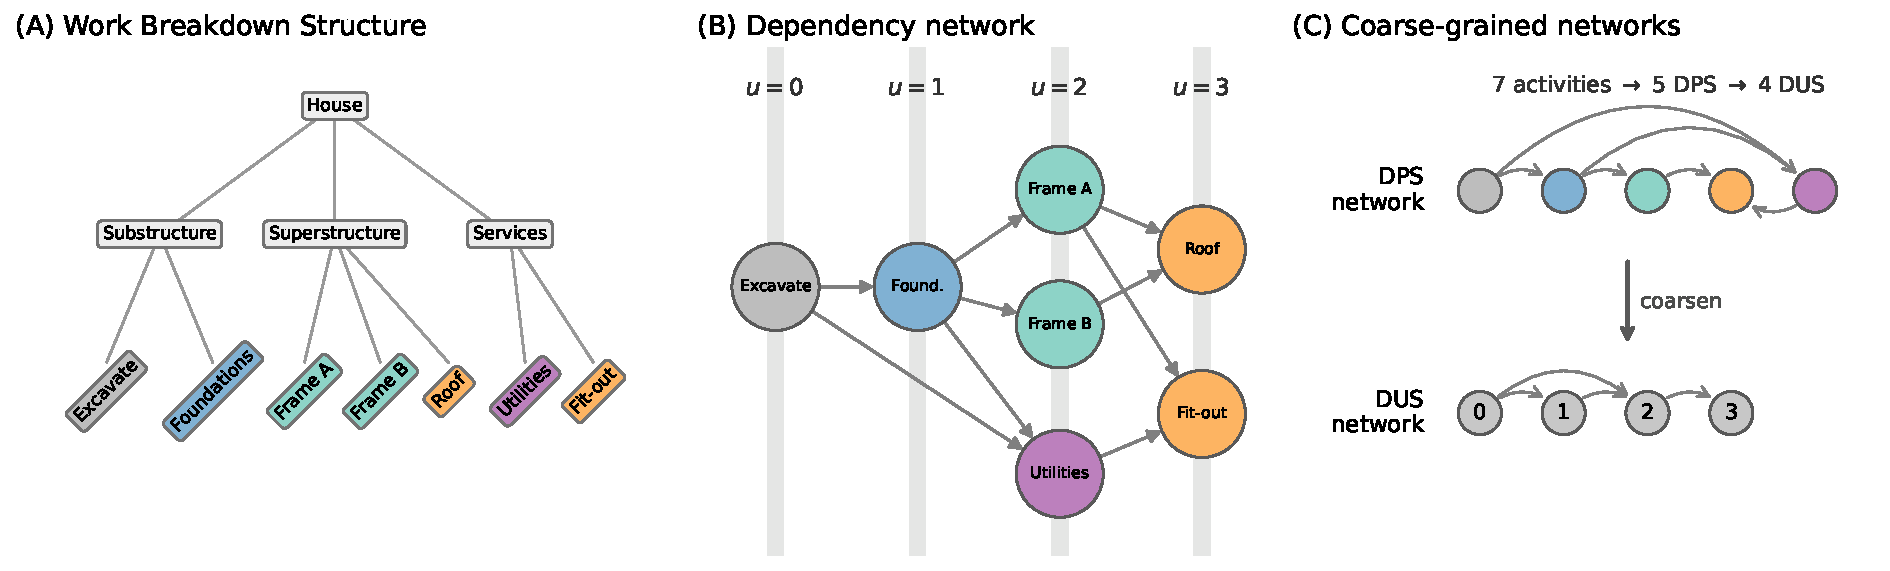
\includegraphics[width=\linewidth]{fig1.pdf}
\caption{The two coarse-grainings, illustrated on a seven-activity project. (A) A Work Breakdown Structure: the project is \DIFdelbeginFL \DIFdelFL{recursively }\DIFdelendFL divided \DIFaddbeginFL \DIFaddFL{recursively }\DIFaddendFL into deliverables until the leaves are schedulable activities. (B) The dependency network of those activities. The DUS index $u$ of an activity is the length of the longest chain of dependencies leading to it, shown by the vertical bands. \DIFdelbeginFL \DIFdelFL{Note that the }\DIFdelendFL \DIFaddbeginFL \DIFaddFL{The }\DIFaddendFL dependency from Excavate to Utilities crosses a WBS branch\DIFdelbeginFL \DIFdelFL{boundary}\DIFdelendFL . Colours indicate the DPS class, \DIFdelbeginFL \DIFdelFL{that is, }\DIFdelendFL the set of DUS levels \DIFaddbeginFL \DIFaddFL{occupied by }\DIFaddendFL the activity's predecessors\DIFdelbeginFL \DIFdelFL{occupy: }\DIFdelendFL \DIFaddbeginFL \DIFaddFL{. }\DIFaddendFL Frame A and Frame B share a DUS level and a DPS class\DIFdelbeginFL \DIFdelFL{, whereas }\DIFdelendFL \DIFaddbeginFL \DIFaddFL{. }\DIFaddendFL Utilities \DIFdelbeginFL \DIFdelFL{shares their }\DIFdelendFL \DIFaddbeginFL \DIFaddFL{is in the same }\DIFaddendFL DUS level but \DIFdelbeginFL \DIFdelFL{forms }\DIFdelendFL \DIFaddbeginFL \DIFaddFL{in }\DIFaddendFL a separate DPS class\DIFaddbeginFL \DIFaddFL{, }\DIFaddendFL because it also depends on level $0$. (C) The \DIFdelbeginFL \DIFdelFL{two }\DIFdelendFL coarse-grained networks obtained by collapsing the dependency network onto DPS classes and onto DUS levels. \DIFdelbeginFL \DIFdelFL{Seven }\DIFdelendFL \DIFaddbeginFL \DIFaddFL{The seven }\DIFaddendFL activities reduce to five DPS classes and four DUS levels.}
\label{schematic}
\end{figure}

\section*{Results}

\subsection*{Dependency Uprise Structure}

We assign \DIFdelbegin \DIFdel{every }\DIFdelend \DIFaddbegin \DIFadd{each }\DIFaddend activity an integer that \DIFdelbegin \DIFdel{measures }\DIFdelend \DIFaddbegin \DIFadd{counts }\DIFaddend how many dependency steps separate it from a starting activity. \DIFdelbegin \DIFdel{We set the DUS index }\DIFdelend \DIFaddbegin \DIFadd{The DUS index is }\DIFaddend $u_i = 0$ for every activity \DIFdelbegin \DIFdel{with no }\DIFdelend \DIFaddbegin \DIFadd{without }\DIFaddend predecessors, and otherwise
%
\begin{equation}
u_i = 1 + \max_{j\in \text{PredecessorsOf}(i)} u_j.
\label{DUS_definition}
\end{equation}
%
\DIFdelbegin \DIFdel{After processing all activities in a }\DIFdelend \DIFaddbegin \DIFadd{Evaluated in }\DIFaddend topological order, $u_i$ \DIFdelbegin \DIFdel{equals }\DIFdelend \DIFaddbegin \DIFadd{is }\DIFaddend the length of the longest chain of dependencies leading to activity $i$. We call it the {\em uprise} index because it \DIFdelbegin \DIFdel{counts }\DIFdelend \DIFaddbegin \DIFadd{measures }\DIFaddend how far the activity \DIFdelbegin \DIFdel{has risen above the start of the project }\DIFdelend \DIFaddbegin \DIFadd{lies above the project start}\DIFaddend , in dependency steps rather than \DIFdelbegin \DIFdel{in }\DIFdelend calendar time.

\DIFdelbegin \DIFdel{Three distinct objectsfollow from Eq. ~(\ref{DUS_definition}), and we keep them separate throughout. }\DIFdelend \DIFaddbegin \DIFadd{We distinguish three objects. }\DIFaddend The {\em DUS index} $u_i$ is an integer attached to each activity. A {\em DUS level} is the set of \DIFdelbegin \DIFdel{all activities sharing one value of }\DIFdelend \DIFaddbegin \DIFadd{activities with the same }\DIFaddend $u_i$. The {\em Dependency Uprise Structure} (DUS) is the \DIFdelbegin \DIFdel{resulting }\DIFdelend partition of the activities into levels. The DUS network, defined in the next section, \DIFdelbegin \DIFdel{is a graph whose nodes are DUS levels }\DIFdelend \DIFaddbegin \DIFadd{has DUS levels as nodes}\DIFaddend .

\DIFdelbegin \DIFdel{By construction, two }\DIFdelend \DIFaddbegin \DIFadd{Two }\DIFaddend activities in the same DUS level are \DIFdelbegin \DIFdel{pairwise incomparablein the dependency DAG --- neither is an ancestor of the other --- }\DIFdelend \DIFaddbegin \DIFadd{incomparable, }\DIFaddend so they can appear in either \DIFdelbegin \DIFdel{relative order within a valid }\DIFdelend \DIFaddbegin \DIFadd{order in a }\DIFaddend topological sort. The converse \DIFdelbegin \DIFdel{does not hold: two }\DIFdelend \DIFaddbegin \DIFadd{is false: }\DIFaddend activities at different depths can also be incomparable\DIFdelbegin \DIFdel{, so the DUS is one specific }\DIFdelend \DIFaddbegin \DIFadd{. The DUS is therefore one }\DIFaddend antichain decomposition of the DAG, \DIFdelbegin \DIFdel{not in general }\DIFdelend \DIFaddbegin \DIFadd{and in general not }\DIFaddend the coarsest one.

\DIFdelbegin \DIFdel{It is worth being explicit about what }\DIFdelend Eq.~(\ref{DUS_definition}) \DIFdelbegin \DIFdel{is not. It is not }\DIFdelend \DIFaddbegin \DIFadd{differs from }\DIFaddend a breadth-first search from the project start, which \DIFdelbegin \DIFdel{would assign each activity }\DIFdelend \DIFaddbegin \DIFadd{gives }\DIFaddend the length of the {\em shortest} path from a starting activity. The two \DIFdelbegin \DIFdel{differ whenever }\DIFdelend \DIFaddbegin \DIFadd{disagree when }\DIFaddend an activity has predecessors at different depths\DIFdelbegin \DIFdel{: in }\DIFdelend \DIFaddbegin \DIFadd{. In }\DIFaddend Figure \ref{schematic}B, a breadth-first search from Excavate \DIFdelbegin \DIFdel{would place }\DIFdelend \DIFaddbegin \DIFadd{places }\DIFaddend Utilities at depth $1$, because Excavate feeds it directly\DIFdelbegin \DIFdel{, whereas }\DIFdelend \DIFaddbegin \DIFadd{. }\DIFaddend Eq.~(\ref{DUS_definition}) places it at $u = 2$, because it \DIFdelbegin \DIFdel{must also wait }\DIFdelend \DIFaddbegin \DIFadd{also waits }\DIFaddend for Foundations. Only the longest-path rule \DIFdelbegin \DIFdel{has the property that matters here, namely that all }\DIFdelend \DIFaddbegin \DIFadd{places all predecessors }\DIFaddend of an activity \DIFdelbegin \DIFdel{'s predecessors lie }\DIFdelend strictly below it, so that the levels are ordered\DIFdelbegin \DIFdel{and every activity is preceded by the entire history it depends on. It is also not a }\DIFdelend \DIFaddbegin \DIFadd{. Eq.~(\ref{DUS_definition}) also differs from a backward }\DIFaddend breadth-first search \DIFdelbegin \DIFdel{backwards from the project-completion }\DIFdelend \DIFaddbegin \DIFadd{from the completion }\DIFaddend node, which would group activities by their remaining depth to the end\DIFdelbegin \DIFdel{rather than by their accumulated depth from the start}\DIFdelend .

\DIFdelbegin \DIFdel{The construction in }\DIFdelend Eq.~(\ref{DUS_definition}) is the layering \DIFdelbegin \DIFdel{used in the first phase }\DIFdelend \DIFaddbegin \DIFadd{step }\DIFaddend of the Sugiyama framework for hierarchical graph drawing \cite{sugiyama1981, healy2013hierarchical} and is \DIFdelbegin \DIFdel{closely }\DIFdelend related to the Coffman--Graham scheduling algorithm \cite{coffmangraham1972}. In project management terms, the DUS index of the final activity is the number of activities on the longest dependency chain, which is the critical path when all \DIFdelbegin \DIFdel{activities have equalduration. The contribution of this paper is not the layering itself but its use as a coarse-graining of }\DIFdelend \DIFaddbegin \DIFadd{durations are equal. The layering itself is therefore not new. What is new here is its use to coarse-grain }\DIFaddend the dependency network, the empirical scaling relations \DIFdelbegin \DIFdel{established }\DIFdelend below, and the finer DPS construction\DIFdelbegin \DIFdel{introduced later}\DIFdelend .

\subsection*{The DUS network}

\DIFdelbegin \DIFdel{Once activities have been grouped into DUS levels, we can collapse the original }\DIFdelend \DIFaddbegin \DIFadd{We collapse the }\DIFaddend dependency network onto \DIFdelbegin \DIFdel{these groups}\DIFdelend \DIFaddbegin \DIFadd{the DUS levels}\DIFaddend . In the resulting DUS network each node is a DUS level, and a weighted edge $U_a \xrightarrow{w_{ab}} U_b$ \DIFdelbegin \DIFdel{records }\DIFdelend \DIFaddbegin \DIFadd{means }\DIFaddend that $w_{ab}$ activity-level dependencies run from \DIFdelbegin \DIFdel{activities in }\DIFdelend level $a$ to \DIFdelbegin \DIFdel{activities in }\DIFdelend level $b$. The DUS network \DIFdelbegin \DIFdel{inherits the directed acyclic structure of the }\DIFdelend \DIFaddbegin \DIFadd{is a DAG, like the }\DIFaddend dependency network. \DIFdelbegin \DIFdel{What is new is the }\DIFdelend \DIFaddbegin \DIFadd{The }\DIFaddend weight $w_{ab}$ \DIFdelbegin \DIFdel{, which }\DIFdelend measures how strongly two \DIFdelbegin \DIFdel{DUS }\DIFdelend levels are coupled.

The simplest DUS network is a chain, for example $U_0 \xrightarrow{w_{01}} U_1 \xrightarrow{w_{12}} U_2$. In general, dependencies may also skip \DIFdelbegin \DIFdel{ahead, linking distant }\DIFdelend levels. A chain through \DIFdelbegin \DIFdel{every level is , however, }\DIFdelend \DIFaddbegin \DIFadd{all levels is }\DIFaddend always present: by Eq.~(\ref{DUS_definition}), every activity has at least one predecessor in the previous \DIFdelbegin \DIFdel{DUS }\DIFdelend level, so $w_{i-1,\,i} \geq 1$. The chain $U_0 \to U_1 \to \cdots \to U_{m-1}$, where $m$ is the number of DUS levels, is \DIFdelbegin \DIFdel{therefore }\DIFdelend \DIFaddbegin \DIFadd{thus }\DIFaddend the longest path in the DUS network. We call it the {\em DUS spine}\DIFdelbegin \DIFdel{, by analogy to the activity-level critical pathwhile avoiding overlap with that term's specific duration-weighted meaning }\DIFdelend \DIFaddbegin \DIFadd{. We avoid the term critical path, which }\DIFaddend in project management \DIFaddbegin \DIFadd{refers to durations}\DIFaddend .

\begin{figure}[t]
\centering
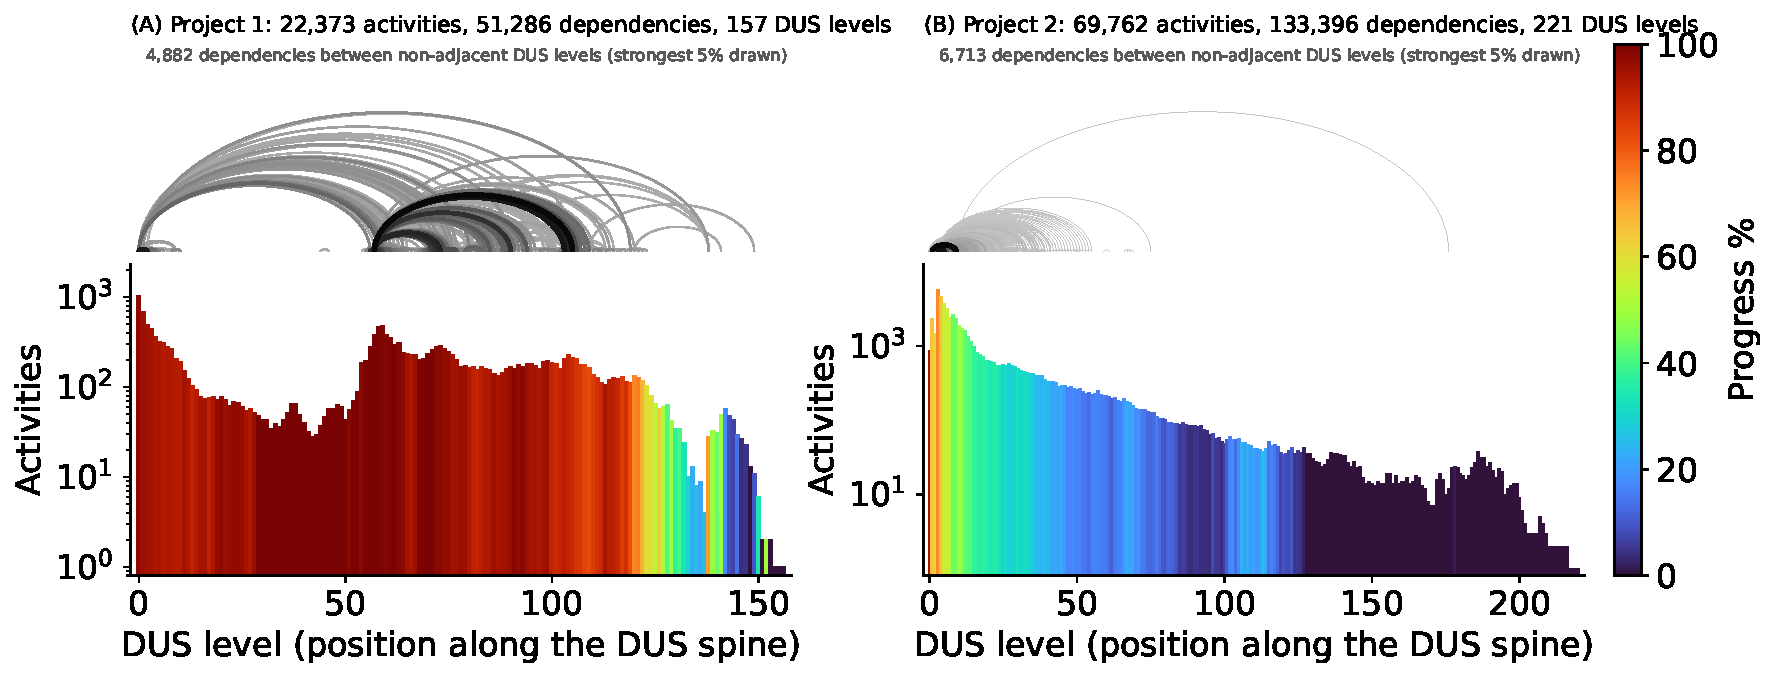
\includegraphics[width=\linewidth]{fig2.pdf}
\caption{DUS profiles of two construction project schedules. The horizontal axis is position along the DUS spine. Bars give the number of activities in each DUS level\DIFdelbeginFL \DIFdelFL{and are }\DIFdelendFL \DIFaddbeginFL \DIFaddFL{, }\DIFaddendFL coloured by the mean Physical Progress Percent of those activities, a standard progress metric in construction. Arcs \DIFdelbeginFL \DIFdelFL{above }\DIFdelendFL show dependencies between non-adjacent DUS levels\DIFdelbeginFL \DIFdelFL{, with }\DIFdelendFL \DIFaddbeginFL \DIFaddFL{; }\DIFaddendFL darker and thicker arcs \DIFdelbeginFL \DIFdelFL{encoding }\DIFdelendFL \DIFaddbeginFL \DIFaddFL{carry }\DIFaddendFL more dependencies\DIFdelbeginFL \DIFdelFL{; only }\DIFdelendFL \DIFaddbeginFL \DIFaddFL{. Only }\DIFaddendFL the strongest 5\% \DIFaddbeginFL \DIFaddFL{of arcs }\DIFaddendFL are drawn\DIFdelbeginFL \DIFdelFL{, since drawing all of them obscures the structure}\DIFdelendFL . Both schedules are included in the public code repository.}
\label{profiles}
\end{figure}

\DIFdelbegin \DIFdel{Because the }\DIFdelend \DIFaddbegin \DIFadd{The }\DIFaddend DUS network has at most a few hundred nodes even for the largest schedules, \DIFdelbegin \DIFdel{it is small enough to draw, which makes it a natural canvas on which to overlay }\DIFdelend \DIFaddbegin \DIFadd{so it can be drawn and used to display }\DIFaddend other project information. Figure \ref{profiles} shows \DIFdelbegin \DIFdel{what we call }\DIFdelend the {\em DUS profile} of two \DIFdelbegin \DIFdel{real construction schedules: the }\DIFdelend \DIFaddbegin \DIFadd{construction schedules. The }\DIFaddend DUS spine runs along the horizontal axis, \DIFdelbegin \DIFdel{the height of each bar }\DIFdelend \DIFaddbegin \DIFadd{bar height }\DIFaddend is the number of activities in \DIFdelbegin \DIFdel{that level, the }\DIFdelend \DIFaddbegin \DIFadd{each level, }\DIFaddend colour encodes progress, and the arcs \DIFdelbegin \DIFdel{above record }\DIFdelend \DIFaddbegin \DIFadd{show }\DIFaddend dependencies that skip levels. \DIFdelbegin \DIFdel{Read this way, a }\DIFdelend \DIFaddbegin \DIFadd{A schedule of }\DIFaddend 22{,}\DIFdelbegin \DIFdel{373-activity schedule }\DIFdelend \DIFaddbegin \DIFadd{373 activities }\DIFaddend becomes a single \DIFdelbegin \DIFdel{legible picture in which one can see }\DIFdelend \DIFaddbegin \DIFadd{figure showing }\DIFaddend where the work is concentrated, how far it has progressed, and where long-range \DIFdelbegin \DIFdel{coupling occurs}\DIFdelend \DIFaddbegin \DIFadd{dependencies occur}\DIFaddend .

\subsection*{Scaling properties}

\begin{table}[t]
\centering
\small
\begin{tabular}{lrcccc}
\hline
 & & Activities & Dependencies & DUS levels & DPS classes \\
Company & Projects & \multicolumn{4}{c}{median [minimum--maximum]} \\
\hline
Blue & 82 & 43{,}167 [83--70{,}503] & 73{,}649 [101--137{,}450] & 170 [32--238] & 3{,}764 [35--9{,}820] \\
Green & 249 & 4{,}520 [37--104{,}981] & 7{,}284 [36--150{,}692] & 108 [17--400] & 1{,}023 [21--8{,}621] \\
Orange & 867 & 9{,}921 [37--64{,}706] & 17{,}117 [55--129{,}067] & 104 [14--571] & 1{,}079 [19--9{,}530] \\
\hline
All & 1198 & 7{,}942 [37--104{,}981] & 13{,}713 [36--150{,}692] & 108 [14--571] & 1{,}070 [19--9{,}820] \\
\hline
\end{tabular}
\caption{Descriptive statistics of the construction project schedules\DIFdelbeginFL \DIFdelFL{analysed here}\DIFdelendFL . The three companies are anonymised and identified by the colours used in Figures~\ref{scaling_size}--\ref{scaling_dps}.}
\label{descriptive}
\end{table}

\begin{figure}[t]
\centering
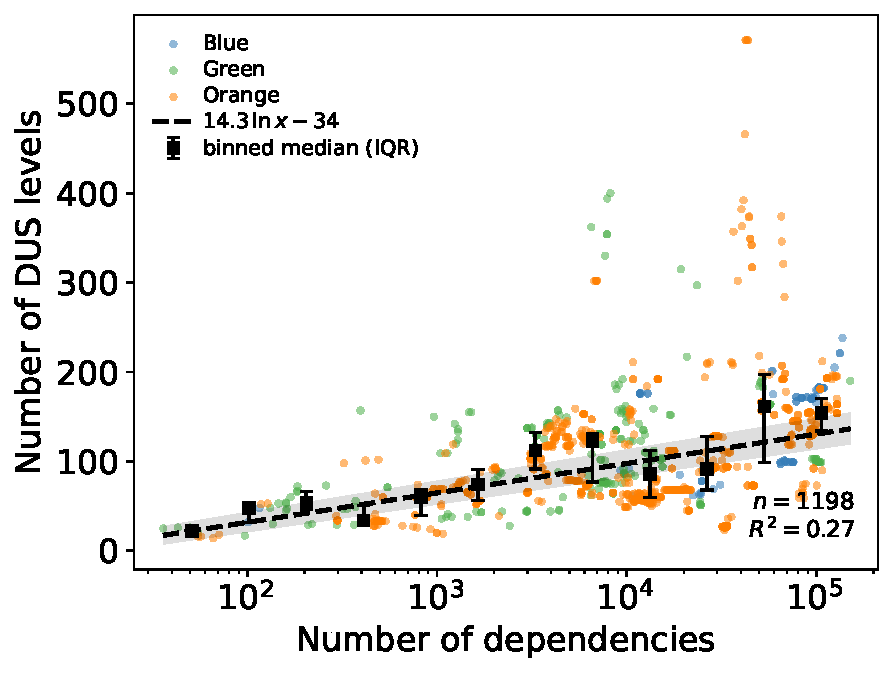
\includegraphics[width=0.62\linewidth]{fig3.pdf}
\caption{The number of DUS levels grows logarithmically with the number of dependencies. Each point is one of 1198 construction projects, coloured by company. The dashed line is the maximum-likelihood fit $m = p\ln x + c$ under multiplicative errors, with $p = 14.3$ and $c = -33.9$; the grey band is the 95\% bootstrap confidence region. Black squares are binned medians with interquartile ranges.}
\label{scaling_size}
\end{figure}

\begin{figure}[t]
\centering
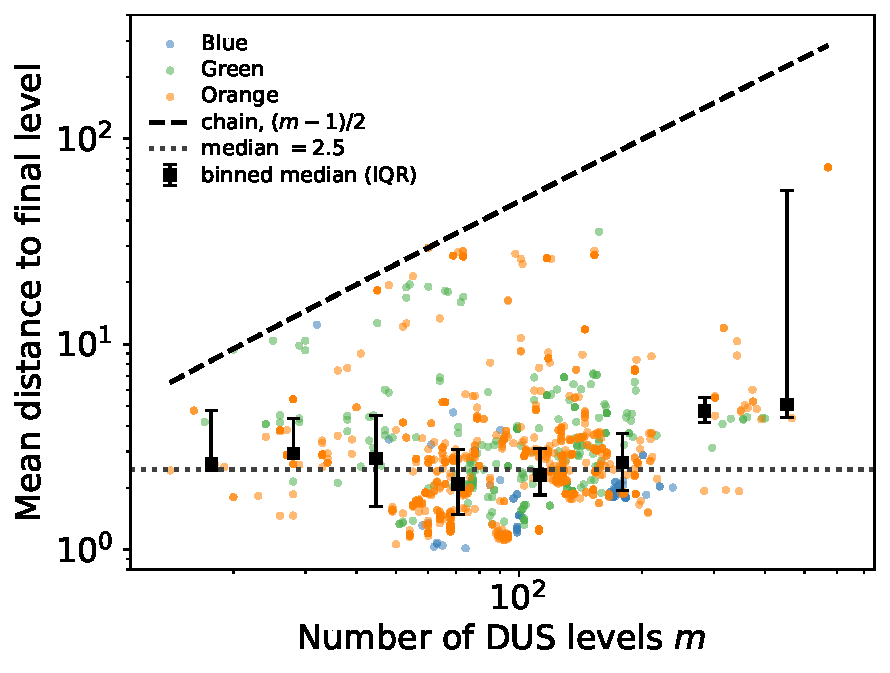
\includegraphics[width=0.62\linewidth]{fig4.pdf}
\caption{Dependencies that skip levels make the DUS network shallow. Mean shortest distance from a DUS level to the final DUS level, against the number of DUS levels $m$. The dashed line is the \DIFdelbeginFL \DIFdelFL{expectation }\DIFdelendFL \DIFaddbeginFL \DIFaddFL{value }\DIFaddendFL $(m-1)/2$ for a pure chain. The distance is \DIFdelbeginFL \DIFdelFL{essentially }\DIFdelendFL \DIFaddbeginFL \DIFaddFL{nearly }\DIFaddendFL independent of $m$, with median $2.5$ (dotted line). Black squares are binned medians with interquartile ranges.}
\label{scaling_distance}
\end{figure}

\DIFdelbegin \DIFdel{To probe how the DUS network scales with project size we }\DIFdelend \DIFaddbegin \DIFadd{We }\DIFaddend collected 1198 schedules from three construction companies, \DIFdelbegin \DIFdel{identified as }\DIFdelend \DIFaddbegin \DIFadd{labelled }\DIFaddend blue, green and orange (see Methods). Table \ref{descriptive} \DIFdelbegin \DIFdel{reports }\DIFdelend \DIFaddbegin \DIFadd{gives }\DIFaddend their descriptive statistics. The \DIFdelbegin \DIFdel{projects span 37 to 104}%DIFDELCMD < {%%%
\DIFdel{,}%DIFDELCMD < }%%%
\DIFdel{981 activities and 36 to 150}%DIFDELCMD < {%%%
\DIFdel{,}%DIFDELCMD < }%%%
\DIFdel{692 dependencies , }\DIFdelend \DIFaddbegin \DIFadd{number of dependencies spans }\DIFaddend close to four orders of magnitude, and the \DIFaddbegin \DIFadd{size ranges of the }\DIFaddend three companies overlap substantially\DIFdelbegin \DIFdel{in size}\DIFdelend .

The number of DUS levels \DIFdelbegin \DIFdel{grows very }\DIFdelend \DIFaddbegin \DIFadd{$m$ grows }\DIFaddend slowly with the number of dependencies \DIFaddbegin \DIFadd{$x$ }\DIFaddend (Figure \ref{scaling_size}). \DIFdelbegin \DIFdel{Because a }\DIFdelend \DIFaddbegin \DIFadd{A }\DIFaddend logarithm and a power law with a small exponent are hard to \DIFdelbegin \DIFdel{tell apart }\DIFdelend \DIFaddbegin \DIFadd{distinguish }\DIFaddend over a finite range\DIFdelbegin \DIFdel{, we }\DIFdelend \DIFaddbegin \DIFadd{. We therefore }\DIFaddend compared four functional forms\DIFdelbegin \DIFdel{--- }\DIFdelend \DIFaddbegin \DIFadd{: }\DIFaddend a one-parameter logarithm, a two-parameter logarithm, a power law and a linear relation\DIFdelbegin \DIFdel{--- each }\DIFdelend \DIFaddbegin \DIFadd{. Each was }\DIFaddend fitted by maximum likelihood \DIFdelbegin \DIFdel{under both additive and multiplicative errors, and selected between them }\DIFdelend \DIFaddbegin \DIFadd{with additive and with multiplicative errors and compared }\DIFaddend by AIC (Methods). The \DIFaddbegin \DIFadd{preferred model is the }\DIFaddend two-parameter logarithm with multiplicative errors\DIFdelbegin \DIFdel{is preferred, with }\DIFdelend \DIFaddbegin \DIFadd{, }\DIFaddend $m = 14.3\ln x - 33.9$\DIFdelbegin \DIFdel{where $x$ is the number of dependencies. It is favoured over }\DIFdelend \DIFaddbegin \DIFadd{. Its AIC is lower by $22$ than that of }\DIFaddend the power law\DIFaddbegin \DIFadd{, }\DIFaddend by \DIFdelbegin \DIFdel{$\Delta\mathrm{AIC} = 22$, over }\DIFdelend \DIFaddbegin \DIFadd{$45$ than that of }\DIFaddend the one-parameter logarithm\DIFaddbegin \DIFadd{, and }\DIFaddend by \DIFdelbegin \DIFdel{$\Delta\mathrm{AIC} = 45$, and over }\DIFdelend \DIFaddbegin \DIFadd{$147$ than that of }\DIFaddend the linear relation\DIFdelbegin \DIFdel{by $\Delta\mathrm{AIC} = 147$; its }\DIFdelend \DIFaddbegin \DIFadd{. Its }\DIFaddend residuals show no detectable heteroscedasticity (Breusch--Pagan $p = 0.07$). The \DIFdelbegin \DIFdel{best-fitting }\DIFdelend \DIFaddbegin \DIFadd{best }\DIFaddend power law has exponent $0.17$, \DIFdelbegin \DIFdel{small enough that the practical distinction from a logarithm matters little }\DIFdelend \DIFaddbegin \DIFadd{which }\DIFaddend over the observed range \DIFdelbegin \DIFdel{. The logarithmic coefficient is $14.3$ with a }\DIFdelend \DIFaddbegin \DIFadd{is close to a logarithm in practice. The }\DIFaddend 95\% bootstrap confidence interval of \DIFaddbegin \DIFadd{the logarithmic coefficient is }\DIFaddend $[13.4, 15.2]$.

The relation \DIFdelbegin \DIFdel{is a statement about the central tendency, not about individual projects: it }\DIFdelend \DIFaddbegin \DIFadd{describes the central trend, not individual projects. It }\DIFaddend explains $27\%$ of the variance in $\ln m$, and at \DIFdelbegin \DIFdel{a given number of dependencies the number of DUS levels }\DIFdelend \DIFaddbegin \DIFadd{fixed $x$ the value of $m$ }\DIFaddend varies by a factor of several. We therefore \DIFdelbegin \DIFdel{describe it as a slow, }\DIFdelend \DIFaddbegin \DIFadd{call it a }\DIFaddend logarithmic growth of the central trend rather than \DIFdelbegin \DIFdel{as }\DIFdelend a scaling law\DIFdelbegin \DIFdel{in the strict sense. Even so, the compression it implies is substantial. Increasing the number of dependencies by a factor of ten }\DIFdelend \DIFaddbegin \DIFadd{. The compression is nonetheless large. A tenfold increase in $x$ }\DIFaddend adds about $33$ DUS levels \DIFdelbegin \DIFdel{regardless of where one starts}\DIFdelend \DIFaddbegin \DIFadd{at any $x$}\DIFaddend , so the DUS network is an exponential compression of the \DIFdelbegin \DIFdel{underlying }\DIFdelend dependency network. \DIFdelbegin \DIFdel{Concretely, the }\DIFdelend \DIFaddbegin \DIFadd{The }\DIFaddend median project in Table \ref{descriptive} has 13{,}713 dependencies and 108 DUS levels.

\DIFdelbegin \DIFdel{Fitting each company separatelygives logarithmic coefficients of }\DIFdelend \DIFaddbegin \DIFadd{Fitted separately, the three companies have logarithmic coefficients }\DIFaddend $15.9$, $16.5$ and $14.6$. \DIFdelbegin \DIFdel{A likelihood ratio test of }\DIFdelend \DIFaddbegin \DIFadd{We compared }\DIFaddend a model with a shared coefficient and company-specific offsets against a model with \DIFdelbegin \DIFdel{fully company-specific parameters }\DIFdelend \DIFaddbegin \DIFadd{all parameters company-specific. A likelihood ratio test }\DIFaddend does not reject the shared coefficient ($\mathrm{LR} = 2.4$, $\mathrm{df} = 2$, $p = 0.30$), and AIC prefers \DIFdelbegin \DIFdel{the shared-coefficient model}\DIFdelend \DIFaddbegin \DIFadd{it}\DIFaddend . The offsets \DIFdelbegin \DIFdel{do }\DIFdelend differ significantly ($\mathrm{LR} = 38.4$, $\mathrm{df} = 2$, $p = 5 \times 10^{-9}$). \DIFdelbegin \DIFdel{So the rate at which levels accumulate with dependencies is common to the three companies at $15.1$ per natural logarithm, while the absolute }\DIFdelend \DIFaddbegin \DIFadd{The three companies thus share the rate $p = 15.1$, while company-specific scheduling practice shifts the }\DIFaddend number of levels\DIFdelbegin \DIFdel{is shifted by company-specific scheduling practice}\DIFdelend .

\DIFdelbegin \DIFdel{A second question is how far apart, on average, two DUS levels are in the network. If a project had no dependencies outside the DUS spine, the }\DIFdelend \DIFaddbegin \DIFadd{We next measured the }\DIFaddend mean shortest distance \DIFdelbegin \DIFdel{from a }\DIFdelend \DIFaddbegin \DIFadd{$L$ from a DUS }\DIFaddend level to the final \DIFdelbegin \DIFdel{one would be exactly $(m-1)/2$. Real projects fall }\DIFdelend \DIFaddbegin \DIFadd{level. Without dependencies outside the spine, $L = (m-1)/2$. Real projects lie }\DIFaddend far below this \DIFdelbegin \DIFdel{expectation }\DIFdelend \DIFaddbegin \DIFadd{value }\DIFaddend (Figure \ref{scaling_distance})\DIFdelbegin \DIFdel{: the median distance }\DIFdelend \DIFaddbegin \DIFadd{. The median $L$ }\DIFaddend is $2.5$ levels, with \DIFdelbegin \DIFdel{an interquartile range of }\DIFdelend \DIFaddbegin \DIFadd{interquartile range }\DIFaddend $[1.9, 3.6]$\DIFdelbegin \DIFdel{, and }\DIFdelend \DIFaddbegin \DIFadd{. In }\DIFaddend $99.8\%$ of projects \DIFdelbegin \DIFdel{lie below the chain expectation, at a median of }\DIFdelend \DIFaddbegin \DIFadd{$L$ is below $(m-1)/2$, and the median ratio is }\DIFaddend $4.6\%$\DIFdelbegin \DIFdel{of it. More striking than the gap is the near-absence of growth. Binned }\DIFdelend \DIFaddbegin \DIFadd{. $L$ also barely grows with $m$. The binned }\DIFaddend medians are $3.4$ \DIFdelbegin \DIFdel{for projects with fewer than }\DIFdelend \DIFaddbegin \DIFadd{below }\DIFaddend $50$ levels, $2.3$ \DIFdelbegin \DIFdel{for }\DIFdelend \DIFaddbegin \DIFadd{between }\DIFaddend $50$ \DIFdelbegin \DIFdel{to }\DIFdelend \DIFaddbegin \DIFadd{and }\DIFaddend $150$ levels, and $2.7$ above $150$ levels, \DIFdelbegin \DIFdel{even though }\DIFdelend \DIFaddbegin \DIFadd{while }\DIFaddend $m$ ranges from $14$ to $571$. The rank correlation between \DIFdelbegin \DIFdel{the two is small though }\DIFdelend \DIFaddbegin \DIFadd{$L$ and $m$ is small but }\DIFaddend nominally significant ($\rho = 0.10$, $p = 8 \times 10^{-4}$\DIFdelbegin \DIFdel{, $n = 1198$). Applying the model selection procedure used }\DIFdelend \DIFaddbegin \DIFadd{). With the same model selection as }\DIFaddend above, a weakly increasing linear relation is \DIFdelbegin \DIFdel{in fact }\DIFdelend preferred over a \DIFdelbegin \DIFdel{strictly constant one }\DIFdelend \DIFaddbegin \DIFadd{constant }\DIFaddend ($\Delta\mathrm{AIC} = 20$), with slope $0.0041$ per level (95\% CI $[0.0018, 0.0062]$). \DIFdelbegin \DIFdel{The growth this implies }\DIFdelend \DIFaddbegin \DIFadd{This growth }\DIFaddend is negligible in practice\DIFdelbegin \DIFdel{: across the entire }\DIFdelend \DIFaddbegin \DIFadd{. Over the }\DIFaddend observed range the fitted \DIFdelbegin \DIFdel{mean distance rises only from $2.5$ to $4.7$, }\DIFdelend \DIFaddbegin \DIFadd{$L$ rises by }\DIFaddend a factor of $1.9$, \DIFdelbegin \DIFdel{while the number of levels grows }\DIFdelend \DIFaddbegin \DIFadd{from $2.5$ to $4.7$, while $m$ rises }\DIFaddend by a factor of $41$.

\DIFdelbegin \DIFdel{The reason is that many dependencies act as shortcuts , linking levels that are far apart along }\DIFdelend \DIFaddbegin \DIFadd{$L$ is small because many dependencies are shortcuts between levels far apart on }\DIFaddend the spine (\DIFdelbegin \DIFdel{see the }\DIFdelend arcs in Figure \ref{profiles}). \DIFdelbegin \DIFdel{This is the mechanism that produces short paths in }\DIFdelend \DIFaddbegin \DIFadd{Shortcuts also produce the short paths of }\DIFaddend small-world networks \cite{watts98}\DIFdelbegin \DIFdel{, and it answers a question a project manager might ask directly: }\DIFdelend \DIFaddbegin \DIFadd{. For a project manager this means that }\DIFaddend a schedule with 500 DUS levels is not 500 steps deep\DIFdelbegin \DIFdel{in any practical sense, because a handful of }\DIFdelend \DIFaddbegin \DIFadd{: a few }\DIFaddend long-range dependencies \DIFdelbegin \DIFdel{carry information from almost anywhere }\DIFdelend \DIFaddbegin \DIFadd{connect almost any level }\DIFaddend to the end in two or three steps.

\subsection*{What makes the DUS network shallow}

\begin{figure}[t]
\centering
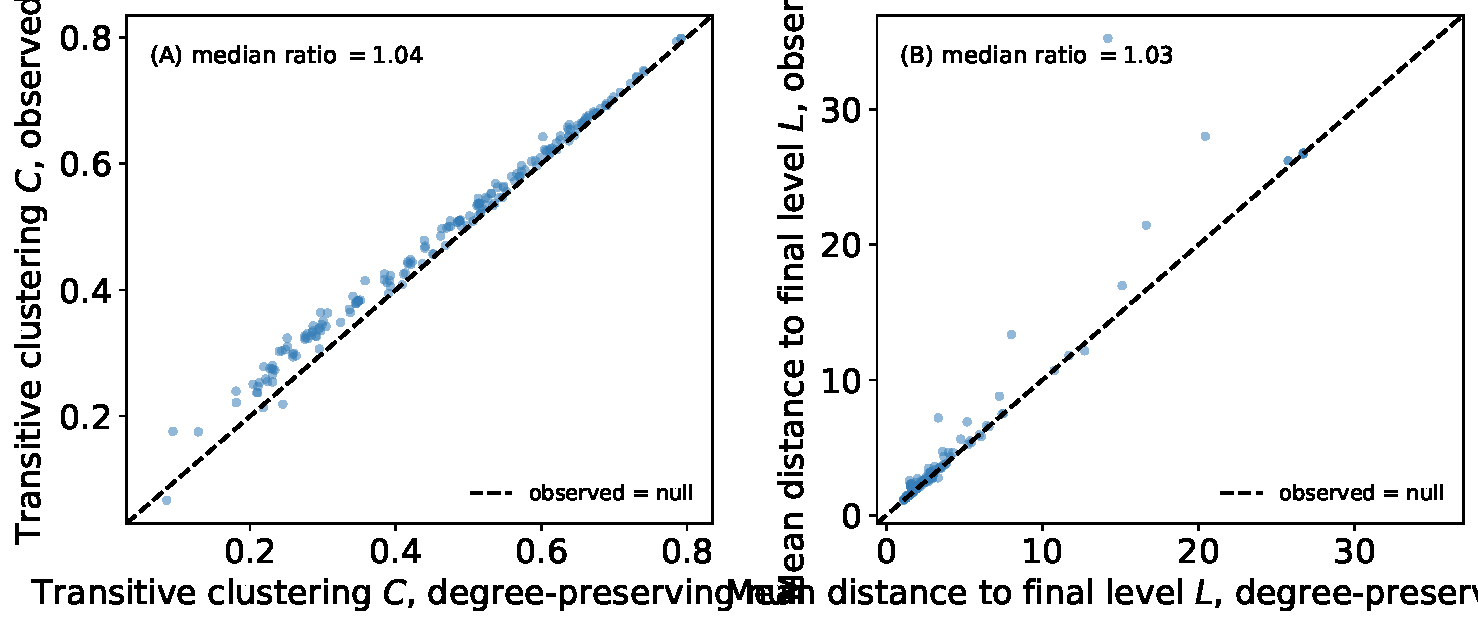
\includegraphics[width=\linewidth]{fig5.pdf}
\caption{The shallowness follows from the degree distributions. Observed versus degree-preserving null values of (A) the transitive clustering coefficient $C$ and (B) the mean distance to the final DUS level $L$, for 198 construction projects. The null \DIFdelbeginFL \DIFdelFL{holds }\DIFdelendFL \DIFaddbeginFL \DIFaddFL{keeps }\DIFaddendFL the DUS spine fixed and rewires the skip dependencies\DIFdelbeginFL \DIFdelFL{while }\DIFdelendFL \DIFaddbeginFL \DIFaddFL{, }\DIFaddendFL preserving \DIFdelbeginFL \DIFdelFL{every level's }\DIFdelendFL \DIFaddbeginFL \DIFaddFL{the }\DIFaddendFL skip in-degree and out-degree \DIFdelbeginFL \DIFdelFL{; each }\DIFdelendFL \DIFaddbeginFL \DIFaddFL{of every level. Each }\DIFaddendFL point is the average over 20 randomisations. Both quantities lie \DIFdelbeginFL \DIFdelFL{essentially on }\DIFdelendFL \DIFaddbeginFL \DIFaddFL{close to }\DIFaddendFL the identity line\DIFdelbeginFL \DIFdelFL{, so randomly reallocating the shortcuts reproduces what is observed}\DIFdelendFL .}
\label{nullmodel}
\end{figure}

\DIFdelbegin \DIFdel{Does this shallowness require the shortcuts to be arranged in some particular way? To find out we compared }\DIFdelend \DIFaddbegin \DIFadd{We tested whether the short distances require a particular arrangement of the shortcuts by comparing }\DIFaddend each DUS network with a degree-preserving null \DIFdelbegin \DIFdel{. Clustering in a DAG cannot be measured with the usual coefficient}\DIFdelend \DIFaddbegin \DIFadd{model. The usual clustering coefficient does not apply to a DAG}\DIFaddend , because a cyclic triangle is impossible\DIFdelbegin \DIFdel{; a }\DIFdelend \DIFaddbegin \DIFadd{. A }\DIFaddend {\em transitive} triangle\DIFdelbegin \DIFdel{is not, since }\DIFdelend \DIFaddbegin \DIFadd{, }\DIFaddend $i \to j$, $j \to k$ and the shortcut $i \to k$\DIFdelbegin \DIFdel{are mutually consistent with acyclicity}\DIFdelend \DIFaddbegin \DIFadd{, is possible}\DIFaddend . We therefore use the transitive clustering coefficient $C$, the fraction of directed two-paths $i \to j \to k$ \DIFdelbegin \DIFdel{that are }\DIFdelend closed by an edge $i \to k$. \DIFdelbegin \DIFdel{It is the admissible member of the directed-triangle family, it is exactly the quantity a shortcut creates, and it is }\DIFdelend \DIFaddbegin \DIFadd{$C$ is }\DIFaddend zero for a pure chain \DIFaddbegin \DIFadd{and increases with the number of shortcuts}\DIFaddend . The null \DIFdelbegin \DIFdel{holds }\DIFdelend \DIFaddbegin \DIFadd{model keeps }\DIFaddend the spine fixed, since Eq.~(\ref{DUS_definition}) forces it\DIFdelbegin \DIFdel{and randomisation should not be free to destroy it}\DIFdelend , and rewires the skip dependencies by double-edge swaps that preserve \DIFdelbegin \DIFdel{every level's }\DIFdelend \DIFaddbegin \DIFadd{the }\DIFaddend skip in-degree and skip out-degree \DIFdelbegin \DIFdel{(see }\DIFdelend \DIFaddbegin \DIFadd{of every level (}\DIFaddend Methods).

Across 198 projects the observed values are \DIFdelbegin \DIFdel{almost exactly }\DIFdelend \DIFaddbegin \DIFadd{close to }\DIFaddend those of the null \DIFaddbegin \DIFadd{model }\DIFaddend (Figure \ref{nullmodel})\DIFdelbegin \DIFdel{: $C/C_{\mathrm{null}} = 1.04$ with an interquartile range of }\DIFdelend \DIFaddbegin \DIFadd{. The median $C/C_{\mathrm{null}}$ is $1.04$ (interquartile range }\DIFaddend $[1.01, 1.10]$\DIFdelbegin \DIFdel{, and $L/L_{\mathrm{null}} = 1.03$ with an interquartile range of }\DIFdelend \DIFaddbegin \DIFadd{) and the median $L/L_{\mathrm{null}}$ is $1.03$ (interquartile range }\DIFaddend $[1.00, 1.08]$\DIFaddbegin \DIFadd{)}\DIFaddend . The short distances \DIFdelbegin \DIFdel{are therefore a consequence of }\DIFdelend \DIFaddbegin \DIFadd{therefore follow from }\DIFaddend the degree distributions of the DUS network\DIFdelbegin \DIFdel{rather than of any special placement of the shortcuts: given how many }\DIFdelend \DIFaddbegin \DIFadd{: given the number of }\DIFaddend long-range dependencies \DIFdelbegin \DIFdel{each level has, putting them anywhere }\DIFdelend \DIFaddbegin \DIFadd{of each level, placing them at random }\DIFaddend reproduces the observed distances. \DIFdelbegin \DIFdel{This closes a link in a mechanistic chain, because the }\DIFdelend \DIFaddbegin \DIFadd{The }\DIFaddend duplication-split model of activity networks \cite{vazquez2023activity} generates degree distributions of \DIFdelbegin \DIFdel{just }\DIFdelend this kind, and \DIFdelbegin \DIFdel{those distributions are what }\DIFdelend the present result shows \DIFdelbegin \DIFdel{to be sufficient .
}\DIFdelend \DIFaddbegin \DIFadd{that these distributions are sufficient for the short distances.
}\DIFaddend 

\DIFdelbegin \DIFdel{It also settles how the small-world question should be posed here.
}\DIFdelend The Watts--Strogatz criterion \DIFdelbegin \DIFdel{asks for clustering substantially in excess }\DIFdelend \DIFaddbegin \DIFadd{for a small world requires clustering well above that }\DIFaddend of a degree-matched null \DIFdelbegin \DIFdel{, and that }\DIFdelend \DIFaddbegin \DIFadd{model. This }\DIFaddend excess is absent \DIFdelbegin \DIFdel{, so the criterion is not the informative test for these networks and we }\DIFdelend \DIFaddbegin \DIFadd{here. We therefore do not use the small-world label and }\DIFaddend state the property directly\DIFdelbegin \DIFdel{instead of invoking the label. The property itself is not in question: the mean distance to the end of the project is }\DIFdelend \DIFaddbegin \DIFadd{: $L$ has median }\DIFaddend $2.5$ levels\DIFdelbegin \DIFdel{where }\DIFdelend \DIFaddbegin \DIFadd{, while }\DIFaddend a chain of the same depth would give up to $285$.

The degree sequence does not \DIFdelbegin \DIFdel{, however, account for everything. Under a stronger randomisation , which }\DIFdelend \DIFaddbegin \DIFadd{explain everything. A stronger randomisation }\DIFaddend preserves the in-degree and out-degree of every {\em activity}, keeps the network acyclic\DIFdelbegin \DIFdel{and then re-derives the DUS decomposition from scratch, the }\DIFdelend \DIFaddbegin \DIFadd{, and recomputes the DUS from scratch. The }\DIFaddend resulting networks are \DIFdelbegin \DIFdel{roughly }\DIFdelend \DIFaddbegin \DIFadd{about }\DIFaddend half as deep as the real ones (median $m/m_{\mathrm{null}} \approx 2$\DIFdelbegin \DIFdel{, a conservative figure since the discrepancy widens }\DIFdelend \DIFaddbegin \DIFadd{). This ratio is a lower bound, since it grows }\DIFaddend with further randomisation\DIFdelbegin \DIFdel{)}\DIFdelend . Real schedules are thus \DIFdelbegin \DIFdel{considerably }\DIFdelend more sequential than \DIFdelbegin \DIFdel{a }\DIFdelend degree-matched random \DIFdelbegin \DIFdel{DAG}\DIFdelend \DIFaddbegin \DIFadd{DAGs}\DIFaddend . The degree distributions determine how short the paths through the DUS network are\DIFdelbegin \DIFdel{; they do not determine how deep it }\DIFdelend \DIFaddbegin \DIFadd{, but not how deep the network }\DIFaddend is.

\subsection*{DUS fine structure}

\begin{figure}[t]
\centering
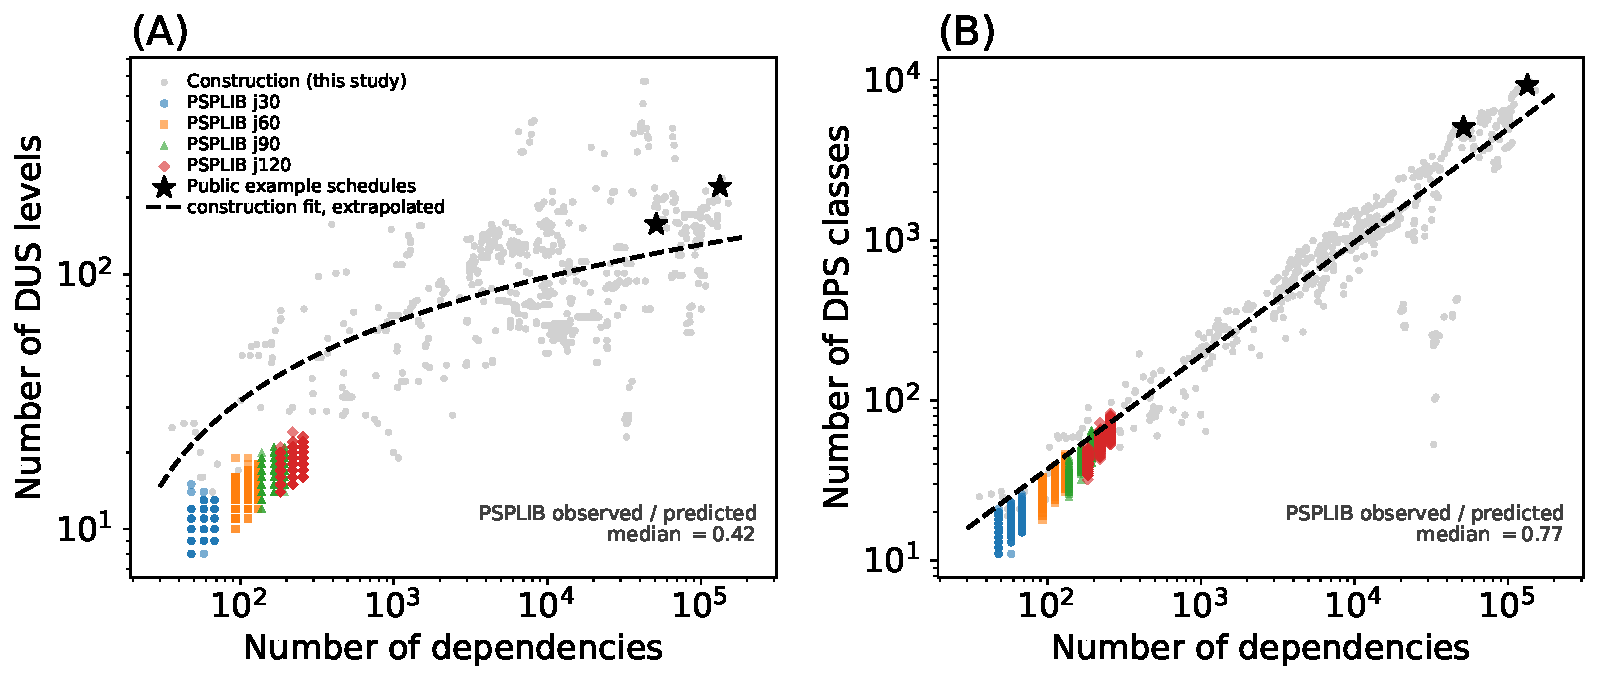
\includegraphics[width=0.62\linewidth]{fig6.pdf}
\caption{The number of DPS classes grows as a sub-linear power law with the number of dependencies. Each point is one of 1198 construction projects, coloured by company. The dashed line is the maximum-likelihood fit $1.42\,x^{0.71}$ under multiplicative errors; the grey band is the 95\% bootstrap confidence region. The dash-dotted line is a linear reference of slope $1$.}
\label{scaling_dps}
\end{figure}

Activities \DIFdelbegin \DIFdel{sharing }\DIFdelend \DIFaddbegin \DIFadd{with }\DIFaddend the same DUS index can be split further according to \DIFdelbegin \DIFdel{which DUS levels their predecessors come from }\DIFdelend \DIFaddbegin \DIFadd{the DUS levels of their predecessors }\DIFaddend (Figure \ref{schematic}B). An activity at $u = i$ \DIFdelbegin \DIFdel{must have }\DIFdelend \DIFaddbegin \DIFadd{has }\DIFaddend at least one predecessor at $u = i-1$\DIFdelbegin \DIFdel{; predecessors at }\DIFdelend \DIFaddbegin \DIFadd{, and may have predecessors at any of }\DIFaddend $u = 0, \ldots, i-2$\DIFdelbegin \DIFdel{are optional}\DIFdelend . Each of \DIFdelbegin \DIFdel{the }\DIFdelend \DIFaddbegin \DIFadd{these }\DIFaddend $i-1$ optional levels \DIFdelbegin \DIFdel{can be }\DIFdelend \DIFaddbegin \DIFadd{is }\DIFaddend either present or absent, \DIFdelbegin \DIFdel{giving $2^{i-1}$ distinguishable predecessor patternsat the }\DIFdelend \DIFaddbegin \DIFadd{so level }\DIFaddend $i$ \DIFdelbegin \DIFdel{-th level}\DIFdelend \DIFaddbegin \DIFadd{admits $2^{i-1}$ predecessor patterns}\DIFaddend . Activities at $u = 0$ have no predecessors, and those at $u = 1$ \DIFdelbegin \DIFdel{draw exclusively from }\DIFdelend \DIFaddbegin \DIFadd{have predecessors only at }\DIFaddend $u = 0$, so neither \DIFaddbegin \DIFadd{level }\DIFaddend can be split\DIFdelbegin \DIFdel{further}\DIFdelend .

We call the resulting partition the {\em Dependency Predecessor Structure} (DPS)\DIFdelbegin \DIFdel{of the network}\DIFdelend , and each \DIFdelbegin \DIFdel{of its parts }\DIFdelend \DIFaddbegin \DIFadd{part }\DIFaddend a DPS class. As \DIFdelbegin \DIFdel{with }\DIFdelend \DIFaddbegin \DIFadd{for }\DIFaddend the DUS, we distinguish the DPS index of an activity, the DPS class as a set of activities, the DPS as the partition, and the DPS network defined below. \DIFdelbegin \DIFdel{These groupings are related to what mathematicians call }\DIFdelend \DIFaddbegin \DIFadd{The DPS is related to }\DIFaddend {\em graph fibrations} \cite{boldi2002fibration, morone2020fibrations}\DIFdelbegin \DIFdel{: two }\DIFdelend \DIFaddbegin \DIFadd{. Two }\DIFaddend activities in the same DPS class have \DIFdelbegin \DIFdel{predecessor sets that occupy the same levels, }\DIFdelend \DIFaddbegin \DIFadd{predecessors in the same set of levels. This is }\DIFaddend a local symmetry of the kind \DIFdelbegin \DIFdel{that fibrationsformalise and that has }\DIFdelend \DIFaddbegin \DIFadd{formalised by fibrations, which have }\DIFaddend been used to find building blocks \DIFdelbegin \DIFdel{in }\DIFdelend \DIFaddbegin \DIFadd{of }\DIFaddend biological networks. \DIFdelbegin \DIFdel{Restricting to DAGs simplifies matters, because }\DIFdelend \DIFaddbegin \DIFadd{In a DAG }\DIFaddend each class can be labelled by a single integer. We set $f_i = 0$ when $u_i = 0$ and otherwise
%
\begin{equation}
f_i= \sum_{k=0}^{u_i - 2} b_{ik}\, 2^{k} + 2^{u_i - 1}
\label{dps_definition}
\end{equation}
%
where $b_{ik}=1$ if activity $i$ has at least one predecessor in DUS level $k$ and $b_{ik}=0$ otherwise. The integer $f_i$ \DIFdelbegin \DIFdel{should be read as }\DIFdelend \DIFaddbegin \DIFadd{is }\DIFaddend a categorical label\DIFdelbegin \DIFdel{, not a metric: numerical proximity of two }\DIFdelend \DIFaddbegin \DIFadd{: close values of }\DIFaddend $f_i$ \DIFdelbegin \DIFdel{values does not imply similarity of their }\DIFdelend \DIFaddbegin \DIFadd{do not imply similar }\DIFaddend predecessor patterns.

\DIFdelbegin \DIFdel{As before, we collapse }\DIFdelend \DIFaddbegin \DIFadd{Collapsing }\DIFaddend the dependency network onto \DIFdelbegin \DIFdel{its DPS classes to obtain }\DIFdelend \DIFaddbegin \DIFadd{DPS classes gives }\DIFaddend the DPS network\DIFdelbegin \DIFdel{: each }\DIFdelend \DIFaddbegin \DIFadd{. Each }\DIFaddend node is a DPS class, and a weighted edge $F_a \xrightarrow{w_{ab}} F_b$ \DIFdelbegin \DIFdel{records }\DIFdelend \DIFaddbegin \DIFadd{counts }\DIFaddend the $w_{ab}$ activity-level dependencies between \DIFdelbegin \DIFdel{them}\DIFdelend \DIFaddbegin \DIFadd{two classes}\DIFaddend . Figure \ref{scaling_dps} \DIFdelbegin \DIFdel{plots }\DIFdelend \DIFaddbegin \DIFadd{shows }\DIFaddend the number of DPS classes \DIFdelbegin \DIFdel{in each project }\DIFdelend \DIFaddbegin \DIFadd{$n$ }\DIFaddend against the number of dependencies \DIFdelbegin \DIFdel{. Applying }\DIFdelend \DIFaddbegin \DIFadd{$x$. With }\DIFaddend the same model selection \DIFdelbegin \DIFdel{procedure }\DIFdelend as above, \DIFaddbegin \DIFadd{the preferred model is }\DIFaddend a power law \DIFdelbegin \DIFdel{under multiplicative errorsis preferred, with $1.42\,x^{0.71}$, ahead }\DIFdelend \DIFaddbegin \DIFadd{with multiplicative errors, $n = 1.42\,x^{0.71}$. Its AIC is lower by $269$ than that }\DIFaddend of the linear relation \DIFaddbegin \DIFadd{and }\DIFaddend by \DIFdelbegin \DIFdel{$\Delta\mathrm{AIC} = 269$ and }\DIFdelend \DIFaddbegin \DIFadd{$1310$ than that of }\DIFaddend the two-parameter logarithm\DIFdelbegin \DIFdel{by $\Delta\mathrm{AIC} = 1310$. The exponent is $0.709$ with a }\DIFdelend \DIFaddbegin \DIFadd{. The }\DIFaddend 95\% bootstrap confidence interval of \DIFaddbegin \DIFadd{the exponent is }\DIFaddend $[0.692, 0.724]$, \DIFdelbegin \DIFdel{comfortably }\DIFdelend \DIFaddbegin \DIFadd{well }\DIFaddend below $1$, and the fit explains $81\%$ of the variance in \DIFdelbegin \DIFdel{the logarithm}\DIFdelend \DIFaddbegin \DIFadd{$\ln n$}\DIFaddend . The residuals \DIFdelbegin \DIFdel{of this fit }\DIFdelend are heteroscedastic, with more scatter at large \DIFdelbegin \DIFdel{sizes, so }\DIFdelend \DIFaddbegin \DIFadd{$x$; for this reason }\DIFaddend the confidence interval \DIFdelbegin \DIFdel{quoted here }\DIFdelend is a case-resampling bootstrap rather than a nominal standard error. As for the DUS, a shared exponent across \DIFdelbegin \DIFdel{the three }\DIFdelend companies is not rejected ($\mathrm{LR} = 1.1$, $\mathrm{df} = 2$, $p = 0.59$; shared exponent $0.72$), while the prefactors differ ($p = 4 \times 10^{-6}$).

The \DIFdelbegin \DIFdel{growth is therefore sub-linear }\DIFdelend \DIFaddbegin \DIFadd{DPS network therefore grows sub-linearly }\DIFaddend but much faster than \DIFdelbegin \DIFdel{logarithmic, placing the DPS network between the original }\DIFdelend \DIFaddbegin \DIFadd{logarithmically, and its size lies between those of the }\DIFaddend dependency network and the \DIFdelbegin \DIFdel{much smaller }\DIFdelend DUS network. The \DIFdelbegin \DIFdel{theoretical }\DIFdelend bound $2^{i-1}$ on the number of patterns at level $i$ is \DIFdelbegin \DIFdel{loose in practice by an enormous margin: a }\DIFdelend \DIFaddbegin \DIFadd{far from reached. A }\DIFaddend project with 100 DUS levels could \DIFdelbegin \DIFdel{in principle realise }\DIFdelend \DIFaddbegin \DIFadd{have }\DIFaddend more than $10^{29}$ classes\DIFdelbegin \DIFdel{and instead realises }\DIFdelend \DIFaddbegin \DIFadd{, but has }\DIFaddend of order $10^{3}$. Most \DIFdelbegin \DIFdel{predecessor patterns that are combinatorially possible simply }\DIFdelend \DIFaddbegin \DIFadd{combinatorially possible predecessor patterns }\DIFaddend do not occur in real schedules.

\subsection*{Replication on public data}

\begin{figure}[t]
\centering
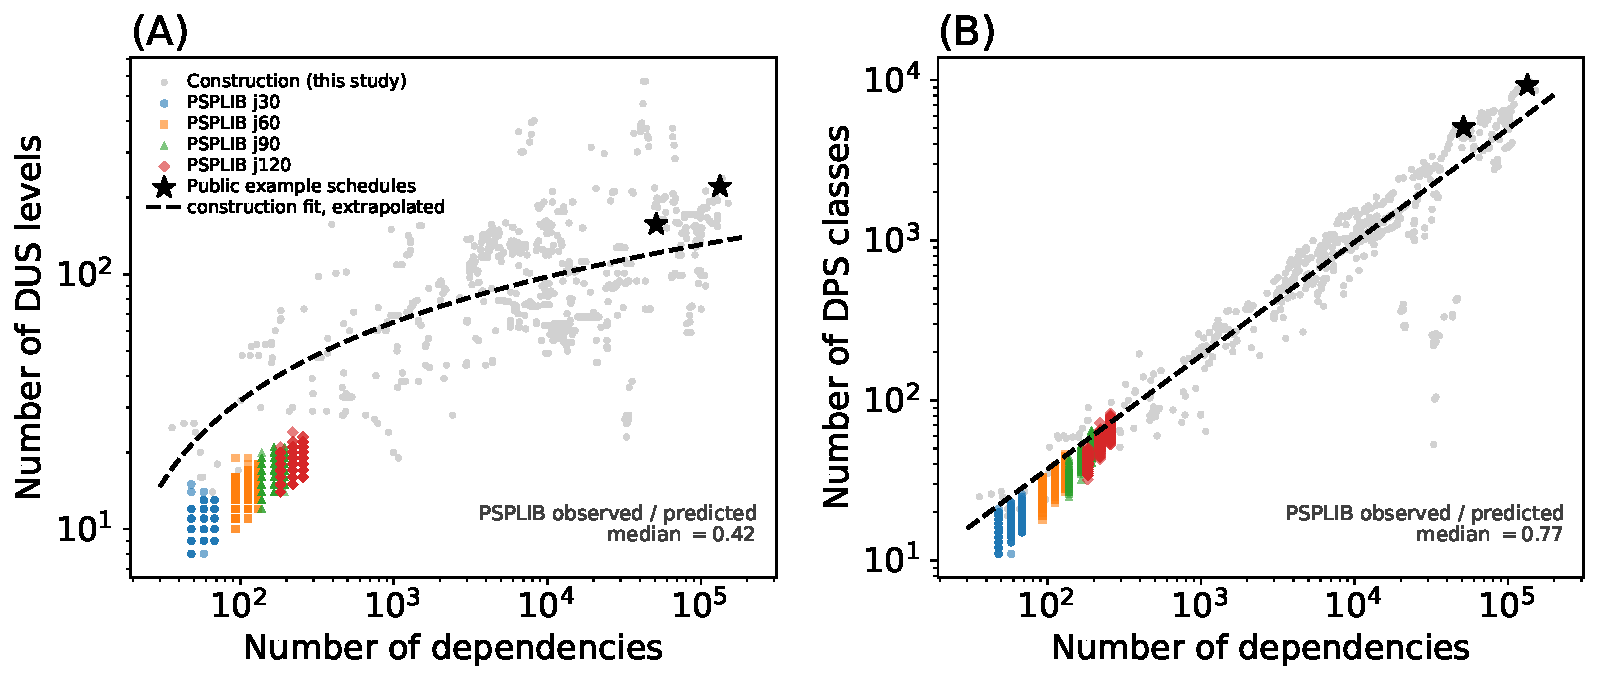
\includegraphics[width=\linewidth]{fig7.pdf}
\caption{Replication on public benchmark instances. (A) Number of DUS levels and (B) number of DPS classes against the number of dependencies, for 2040 single-mode PSPLIB instances (coloured), the 1198 construction schedules of this study (grey), and the two anonymised \DIFdelbeginFL \DIFdelFL{real }\DIFdelendFL schedules distributed with the code repository (stars). Dashed lines are the fits to the construction data, evaluated two orders of magnitude below the median project size on which they were estimated. Only $2.4\%$ of the construction projects are as small as the largest PSPLIB instance.}
\label{public}
\end{figure}

The construction schedules \DIFdelbegin \DIFdel{analysed here }\DIFdelend are proprietary. To make the \DIFdelbegin \DIFdel{central }\DIFdelend \DIFaddbegin \DIFadd{main }\DIFaddend results reproducible from public data, we repeated the analysis on the 2040 single-mode instances of PSPLIB \cite{kolisch1997psplib}, the standard benchmark library for resource-constrained project scheduling, and on the two anonymised \DIFdelbegin \DIFdel{real }\DIFdelend schedules distributed with our code (Figure \ref{public}).

PSPLIB instances are much smaller than real construction schedules. They \DIFdelbegin \DIFdel{contain 32 to 122 activities and }\DIFdelend \DIFaddbegin \DIFadd{have }\DIFaddend 48 to 257 dependencies, come in only four activity counts, and span \DIFdelbegin \DIFdel{barely }\DIFdelend \DIFaddbegin \DIFadd{about }\DIFaddend half a decade in size\DIFdelbegin \DIFdel{; their dependency range overlaps only the extreme lower tail of ours, since just }\DIFdelend \DIFaddbegin \DIFadd{. Only }\DIFaddend $2.4\%$ of our construction projects ($29$ of $1198$) are \DIFdelbegin \DIFdel{that small. Model selection within PSPLIB alone}\DIFdelend \DIFaddbegin \DIFadd{this small. Within PSPLIB alone, model selection }\DIFaddend favours a power law for the number of DUS levels and a linear relation for the number of DPS classes, \DIFdelbegin \DIFdel{which are not the forms selected on the }\DIFdelend \DIFaddbegin \DIFadd{unlike the }\DIFaddend construction data. \DIFdelbegin \DIFdel{Over }\DIFdelend \DIFaddbegin \DIFadd{With four distinct sizes over }\DIFaddend so narrow a range, \DIFdelbegin \DIFdel{and with only four distinct sizes, }\DIFdelend we do not \DIFdelbegin \DIFdel{read }\DIFdelend \DIFaddbegin \DIFadd{take }\DIFaddend this as evidence about functional form. We use PSPLIB instead \DIFdelbegin \DIFdel{for the question it can answer, which is }\DIFdelend \DIFaddbegin \DIFadd{to test }\DIFaddend whether the construction relations transfer to independent data at \DIFdelbegin \DIFdel{a size }\DIFdelend \DIFaddbegin \DIFadd{sizes }\DIFaddend where they were barely constrained.

For the DPS \DIFdelbegin \DIFdel{the answer is yes}\DIFdelend \DIFaddbegin \DIFadd{they do}\DIFaddend . The construction power law, evaluated two orders of magnitude below the median project \DIFdelbegin \DIFdel{on which it was estimated}\DIFdelend \DIFaddbegin \DIFadd{size}\DIFaddend , predicts the PSPLIB values \DIFdelbegin \DIFdel{to }\DIFdelend \DIFaddbegin \DIFadd{with }\DIFaddend a median observed/predicted ratio of $0.77$ (Figure \ref{public}B)\DIFdelbegin \DIFdel{, and the }\DIFdelend \DIFaddbegin \DIFadd{. A }\DIFaddend power law fitted \DIFdelbegin \DIFdel{within PSPLIB alone , though not the form AIC prefers there, }\DIFdelend \DIFaddbegin \DIFadd{to PSPLIB alone }\DIFaddend has exponent $0.86$, also sub-linear\DIFaddbegin \DIFadd{, although AIC does not prefer it there}\DIFaddend . For the DUS \DIFdelbegin \DIFdel{the answer is no: the }\DIFdelend \DIFaddbegin \DIFadd{they do not. The }\DIFaddend construction logarithm over-predicts the PSPLIB values by more than a factor of two\DIFdelbegin \DIFdel{(}\DIFdelend \DIFaddbegin \DIFadd{, with a }\DIFaddend median observed/predicted ratio \DIFaddbegin \DIFadd{of }\DIFaddend $0.42$ \DIFdelbegin \DIFdel{, }\DIFdelend \DIFaddbegin \DIFadd{(}\DIFaddend Figure \ref{public}A). The logarithmic relation \DIFdelbegin \DIFdel{should therefore be read as a description of }\DIFdelend \DIFaddbegin \DIFadd{thus describes }\DIFaddend large construction schedules \DIFdelbegin \DIFdel{rather than as }\DIFdelend \DIFaddbegin \DIFadd{and is not }\DIFaddend a universal law, which is a further reason \DIFdelbegin \DIFdel{to avoid the term scaling lawfor it}\DIFdelend \DIFaddbegin \DIFadd{not to call it a scaling law}\DIFaddend . The qualitative \DIFdelbegin \DIFdel{claims do }\DIFdelend \DIFaddbegin \DIFadd{result does }\DIFaddend transfer: PSPLIB DUS networks are also shallow\DIFdelbegin \DIFdel{, with a median distance to the final level of }\DIFdelend \DIFaddbegin \DIFadd{. Their median $L$ is }\DIFaddend $2.1$, \DIFaddbegin \DIFadd{and every instance lies }\DIFaddend below the chain \DIFdelbegin \DIFdel{expectation in $100\%$ of instances}\DIFdelend \DIFaddbegin \DIFadd{value}\DIFaddend .

\section*{Discussion}

Dependency networks admit two \DIFdelbegin \DIFdel{natural }\DIFdelend higher-level representations\DIFdelbegin \DIFdel{forming }\DIFdelend \DIFaddbegin \DIFadd{, which form }\DIFaddend a chain of \DIFdelbegin \DIFdel{progressively coarser }\DIFdelend \DIFaddbegin \DIFadd{increasingly coarse }\DIFaddend views, $\textit{Activity} \to \textit{DPS} \to \textit{DUS}$. For construction \DIFdelbegin \DIFdel{project }\DIFdelend schedules, the DPS \DIFdelbegin \DIFdel{provides }\DIFdelend \DIFaddbegin \DIFadd{is }\DIFaddend a sub-linear coarse-graining and the DUS an exponential one.

\DIFdelbegin \DIFdel{The practical value of these constructions to project managementis that they }\DIFdelend \DIFaddbegin \DIFadd{For project management, these constructions }\DIFaddend give a view of the schedule that the WBS \DIFdelbegin \DIFdel{cannot}\DIFdelend \DIFaddbegin \DIFadd{does not}\DIFaddend . A WBS reports progress by deliverable\DIFdelbegin \DIFdel{; the }\DIFdelend \DIFaddbegin \DIFadd{. The }\DIFaddend DUS reports it by logical depth, which \DIFdelbegin \DIFdel{is what }\DIFdelend determines what can start next. \DIFdelbegin \DIFdel{Three usesfollow directly}\DIFdelend \DIFaddbegin \DIFadd{We see three uses}\DIFaddend . First, reporting\DIFdelbegin \DIFdel{and tracking}\DIFdelend : the DUS profile \DIFdelbegin \DIFdel{of Figure \ref{profiles}compresses }\DIFdelend \DIFaddbegin \DIFadd{(Figure \ref{profiles}) reduces }\DIFaddend a schedule of tens of thousands of activities \DIFdelbegin \DIFdel{into a picture with of order a }\DIFdelend \DIFaddbegin \DIFadd{to about a }\DIFaddend hundred nodes, on which progress, cost or risk can be \DIFdelbegin \DIFdel{overlaid, and in which }\DIFdelend \DIFaddbegin \DIFadd{displayed, and }\DIFaddend a stalled level or \DIFdelbegin \DIFdel{an unusually }\DIFdelend \DIFaddbegin \DIFadd{a }\DIFaddend large concentration of work is \DIFdelbegin \DIFdel{immediately visible}\DIFdelend \DIFaddbegin \DIFadd{easy to see}\DIFaddend . Second, diagnosis: the arcs in Figure \ref{profiles} are dependencies that jump many levels, and \DIFdelbegin \DIFdel{these are exactly the links whose delay propagates furthest; they are candidates for scrutiny because a long-range dependency is often either a genuine }\DIFdelend \DIFaddbegin \DIFadd{their delays propagate furthest. Each such dependency is either a real }\DIFaddend structural constraint or an artefact of how the schedule was built\DIFaddbegin \DIFadd{, and is worth checking}\DIFaddend . Third, \DIFdelbegin \DIFdel{as an input to risk models, since a coarse-grained network with }\DIFdelend \DIFaddbegin \DIFadd{risk modelling: a network of }\DIFaddend a hundred nodes \DIFdelbegin \DIFdel{is tractable for simulation where one with }\DIFdelend \DIFaddbegin \DIFadd{can be simulated where one of }\DIFaddend a hundred thousand \DIFdelbegin \DIFdel{is not. That }\DIFdelend \DIFaddbegin \DIFadd{cannot. Because }\DIFaddend the compression is deterministic and \DIFdelbegin \DIFdel{parameter-free matters here: }\DIFdelend \DIFaddbegin \DIFadd{has no parameters, }\DIFaddend two planners applying it to the same schedule \DIFdelbegin \DIFdel{obtain the same answer, which is not true of }\DIFdelend \DIFaddbegin \DIFadd{get the same result. This is not the case for }\DIFaddend clustering methods that depend on an objective function or a random seed.

\DIFdelbegin \DIFdel{Three limitationsshould be kept in view. The relations reported here }\DIFdelend \DIFaddbegin \DIFadd{The work has three limitations. First, the relations }\DIFaddend are established on schedules from three companies in one sector, and the \DIFdelbegin \DIFdel{failure of the logarithmic relation to }\DIFdelend \DIFaddbegin \DIFadd{logarithmic relation does not }\DIFaddend extrapolate to PSPLIB\DIFdelbegin \DIFdel{shows that }\DIFdelend \DIFaddbegin \DIFadd{, so }\DIFaddend the coefficients are not universal. \DIFdelbegin \DIFdel{The }\DIFdelend \DIFaddbegin \DIFadd{Second, the }\DIFaddend DUS is one antichain decomposition among many, and we have not shown it \DIFdelbegin \DIFdel{is }\DIFdelend \DIFaddbegin \DIFadd{to be }\DIFaddend optimal by any criterion\DIFdelbegin \DIFdel{; it is justified by being }\DIFdelend \DIFaddbegin \DIFadd{. We use it because it is }\DIFaddend canonical, cheap \DIFdelbegin \DIFdel{and interpretable rather than by an optimality argument. Finally, the null models used here randomise one structure at a time, }\DIFdelend \DIFaddbegin \DIFadd{to compute and easy to interpret. Third, each null model randomises one structure while }\DIFaddend holding either the DUS spine or the activity degree sequence fixed\DIFdelbegin \DIFdel{; they bound }\DIFdelend \DIFaddbegin \DIFadd{. The null models show }\DIFaddend what those constraints alone imply\DIFdelbegin \DIFdel{, and are not a generative account of }\DIFdelend \DIFaddbegin \DIFadd{; they do not explain }\DIFaddend how real schedules \DIFdelbegin \DIFdel{come to have the degree distributionsthey do}\DIFdelend \DIFaddbegin \DIFadd{acquire their degree distributions}\DIFaddend .

\DIFdelbegin \DIFdel{Because the construction is purely topological, the same machinery }\DIFdelend \DIFaddbegin \DIFadd{The construction uses only the network topology, so it }\DIFaddend applies to any system \DIFdelbegin \DIFdel{representable as a directed acyclic graph}\DIFdelend \DIFaddbegin \DIFadd{represented by a DAG}\DIFaddend , including causal networks, ancestries and feedforward neural networks. \DIFdelbegin \DIFdel{Three questionsfollow}\DIFdelend \DIFaddbegin \DIFadd{This raises three questions}\DIFaddend . Do the size relations \DIFdelbegin \DIFdel{observed }\DIFdelend \DIFaddbegin \DIFadd{found }\DIFaddend for construction schedules \DIFdelbegin \DIFdel{carry over to those settings}\DIFdelend \DIFaddbegin \DIFadd{hold in those systems}\DIFaddend , and if the coefficients differ, what do the differences measure? \DIFdelbegin \DIFdel{What features of the underlying }\DIFdelend \DIFaddbegin \DIFadd{Which features of a }\DIFaddend dependency network determine the structure of its DPS and DUS networks? \DIFdelbegin \DIFdel{And since the }\DIFdelend \DIFaddbegin \DIFadd{The }\DIFaddend degree distributions of the DUS network \DIFdelbegin \DIFdel{are enough to produce }\DIFdelend \DIFaddbegin \DIFadd{account for }\DIFaddend its short distances but not its depth\DIFdelbegin \DIFdel{, what generative mechanism fixes }\DIFdelend \DIFaddbegin \DIFadd{; which generative mechanism sets }\DIFaddend the depth? The duplication-split model \cite{vazquez2023activity} is a \DIFdelbegin \DIFdel{natural candidate, since }\DIFdelend \DIFaddbegin \DIFadd{candidate, because }\DIFaddend its split operation creates \DIFdelbegin \DIFdel{sequential structure of exactly the sort the }\DIFdelend \DIFaddbegin \DIFadd{the sequential structure that the }\DIFaddend degree-preserving null \DIFdelbegin \DIFdel{destroys}\DIFdelend \DIFaddbegin \DIFadd{model removes}\DIFaddend .

\section*{Methods}

\subsection*{Dataset}

The construction project schedules \DIFdelbegin \DIFdel{analysed here were drawn }\DIFdelend \DIFaddbegin \DIFadd{were taken }\DIFaddend from the Nodes \& Links database. \DIFdelbegin \DIFdel{Three construction companiesare represented, identified throughout as }\DIFdelend \DIFaddbegin \DIFadd{They come from three construction companies, labelled }\DIFaddend blue, green and orange, \DIFdelbegin \DIFdel{contributing }\DIFdelend \DIFaddbegin \DIFadd{which contribute }\DIFaddend 82, 249 and 867 projects respectively, \DIFdelbegin \DIFdel{for a totalof 1198. Table \ref{descriptive} reports }\DIFdelend \DIFaddbegin \DIFadd{1198 in total. Table \ref{descriptive} gives }\DIFaddend the number of activities, dependencies, DUS levels and DPS classes for each company. One further schedule was excluded because its first DUS level connects directly to every other level, so \DIFdelbegin \DIFdel{that }\DIFdelend its DUS network is a star \DIFdelbegin \DIFdel{rather than a network with a }\DIFdelend \DIFaddbegin \DIFadd{without a }\DIFaddend spine. Activity-level dependencies and Physical Progress Percent values were taken directly from the schedules as recorded in the database.

The public replication uses the four single-mode PSPLIB instance sets j30, j60, j90 and j120 \cite{kolisch1997psplib}\DIFdelbegin \DIFdel{, comprising }\DIFdelend \DIFaddbegin \DIFadd{. These comprise }\DIFaddend 2040 instances of 32, 62, 92 and 122 activities, downloaded from the PSPLIB distribution site. The precedence relations of each instance were \DIFdelbegin \DIFdel{extracted and treated exactly }\DIFdelend \DIFaddbegin \DIFadd{treated }\DIFaddend as the dependencies of a construction schedule.

\subsection*{Computation of the DUS and DPS}

The \DIFdelbegin \DIFdel{DUS index $u_i$ defined in Eq.~(\ref{DUS_definition}) is computed by first sorting the activities }\DIFdelend \DIFaddbegin \DIFadd{activities are first sorted }\DIFaddend into a topological order \DIFdelbegin \DIFdel{using }\DIFdelend \DIFaddbegin \DIFadd{with }\DIFaddend Kahn's algorithm\DIFdelbegin \DIFdel{, then sweeping through that order and applying }\DIFdelend \DIFaddbegin \DIFadd{. }\DIFaddend Eq.~(\ref{DUS_definition}) \DIFaddbegin \DIFadd{is then applied }\DIFaddend to each activity in \DIFdelbegin \DIFdel{turn}\DIFdelend \DIFaddbegin \DIFadd{that order}\DIFaddend . The cost is linear in the number of activities plus the number of dependencies. \DIFdelbegin \DIFdel{The }\DIFdelend \DIFaddbegin \DIFadd{Given $u_i$, the }\DIFaddend DPS index $f_i$ \DIFdelbegin \DIFdel{defined in }\DIFdelend \DIFaddbegin \DIFadd{of }\DIFaddend Eq.~(\ref{dps_definition}) requires \DIFdelbegin \DIFdel{a single additional }\DIFdelend \DIFaddbegin \DIFadd{one more }\DIFaddend pass over the dependencies\DIFdelbegin \DIFdel{once $u_i$ is known}\DIFdelend : for each activity $i$ we record which lower DUS levels its predecessors occupy \DIFdelbegin \DIFdel{, }\DIFdelend and combine these bits \DIFdelbegin \DIFdel{into the integer label given by }\DIFdelend \DIFaddbegin \DIFadd{as in }\DIFaddend Eq.~(\ref{dps_definition}). The DUS and DPS networks are \DIFdelbegin \DIFdel{then }\DIFdelend obtained by collapsing the dependency network onto these labels and \DIFdelbegin \DIFdel{accumulating }\DIFdelend \DIFaddbegin \DIFadd{summing }\DIFaddend edge weights. Distances \DIFdelbegin \DIFdel{within }\DIFdelend \DIFaddbegin \DIFadd{in }\DIFaddend the DUS network are \DIFaddbegin \DIFadd{unweighted directed }\DIFaddend shortest-path \DIFdelbegin \DIFdel{distances in the unweighted directed network}\DIFdelend \DIFaddbegin \DIFadd{distances}\DIFaddend , computed by \DIFdelbegin \DIFdel{a single }\DIFdelend \DIFaddbegin \DIFadd{one }\DIFaddend reverse sweep over the levels.

\subsection*{Null models for the DUS network}

\DIFdelbegin \DIFdel{Two }\DIFdelend \DIFaddbegin \DIFadd{We used two }\DIFaddend degree-preserving randomisations\DIFdelbegin \DIFdel{were used}\DIFdelend , both by double-edge swaps, which
preserve in- and out-degree exactly.

The first randomises the DUS network\DIFdelbegin \DIFdel{itself}\DIFdelend . The spine $U_0 \to U_1 \to \cdots$
is forced by Eq.~(\ref{DUS_definition}) and is held fixed. The \DIFdelbegin \DIFdel{remaining }\DIFdelend skip
dependencies are rewired by \DIFdelbegin \DIFdel{repeatedly }\DIFdelend choosing two of them, $a \to b$ and
$c \to d$, and replacing them by $a \to d$ and $c \to b$ \DIFdelbegin \DIFdel{whenever both results
are still }\DIFdelend \DIFaddbegin \DIFadd{if both new edges
are }\DIFaddend forward skips and neither already exists. This preserves \DIFdelbegin \DIFdel{each level's
}\DIFdelend \DIFaddbegin \DIFadd{the }\DIFaddend skip
in-degree and skip out-degree \DIFdelbegin \DIFdel{and the acyclicity of the network }\DIFdelend \DIFaddbegin \DIFadd{of each level and keeps the network acyclic}\DIFaddend . We
used 20 swap attempts per skip edge and averaged over 20 randomisations per
project\DIFdelbegin \DIFdel{;
the resulting }\DIFdelend \DIFaddbegin \DIFadd{. }\DIFaddend $C$ and $L$ \DIFdelbegin \DIFdel{are unchanged }\DIFdelend \DIFaddbegin \DIFadd{do not change }\DIFaddend between 5 and 80 swap attempts per edge,
so the chain is well mixed.

The second randomises the activity network. A topological order of the observed
DAG is fixed, and pairs of dependencies are swapped \DIFdelbegin \DIFdel{whenever both resulting
edges still }\DIFdelend \DIFaddbegin \DIFadd{if both new edges }\DIFaddend point
forward in that order\DIFdelbegin \DIFdel{, which preserves every activity's }\DIFdelend \DIFaddbegin \DIFadd{. This preserves the }\DIFaddend in- and out-degree \DIFdelbegin \DIFdel{and guarantees the result is }\DIFdelend \DIFaddbegin \DIFadd{of every activity
and keeps the network }\DIFaddend acyclic. The DUS \DIFdelbegin \DIFdel{decomposition }\DIFdelend is then recomputed from scratch. This
randomisation mixes more slowly: the number of DUS levels \DIFdelbegin \DIFdel{is still drifting }\DIFdelend \DIFaddbegin \DIFadd{still drifts }\DIFaddend at 20
swap attempts per edge, and the gap between \DIFdelbegin \DIFdel{the }\DIFdelend observed and randomised networks
widens \DIFdelbegin \DIFdel{as mixingproceeds, so the
}\DIFdelend \DIFaddbegin \DIFadd{with further mixing. The }\DIFaddend ratios reported for it are \DIFdelbegin \DIFdel{conservative }\DIFdelend \DIFaddbegin \DIFadd{therefore lower
}\DIFaddend bounds rather than converged estimates.

\DIFdelbegin \DIFdel{Clustering is measured by the }\DIFdelend \DIFaddbegin \DIFadd{The }\DIFaddend transitive clustering coefficient \DIFdelbegin \DIFdel{, }\DIFdelend \DIFaddbegin \DIFadd{$C$ is }\DIFaddend the number of directed two-paths
$i \to j \to k$ closed by an edge $i \to k$\DIFaddbegin \DIFadd{, }\DIFaddend divided by the number of directed
two-paths. \DIFdelbegin \DIFdel{Distances are }\DIFdelend \DIFaddbegin \DIFadd{$L$ is the mean }\DIFaddend shortest-path \DIFdelbegin \DIFdel{distances }\DIFdelend \DIFaddbegin \DIFadd{distance }\DIFaddend to the final DUS level\DIFdelbegin \DIFdel{, as elsewhere in the paper}\DIFdelend .

\subsection*{Statistical methods}

For each relation we fitted four \DIFdelbegin \DIFdel{candidate }\DIFdelend functional forms: a one-parameter logarithm $y = p\ln x$, a two-parameter logarithm $y = p\ln x + c$, a power law $y = a x^{b}$, and a linear relation $y = ax + b$. Each was fitted by maximum likelihood \DIFdelbegin \DIFdel{under }\DIFdelend \DIFaddbegin \DIFadd{with }\DIFaddend two error structures: additive, $y = f(x) + \varepsilon$\DIFdelbegin \DIFdel{with $\varepsilon \sim N(0,\sigma^2)$}\DIFdelend , and multiplicative, $y = f(x)\,e^{\varepsilon}$\DIFaddbegin \DIFadd{, }\DIFaddend with $\varepsilon \sim N(0,\sigma^2)$ \DIFaddbegin \DIFadd{in both cases}\DIFaddend . The multiplicative log-likelihoods include the Jacobian term $-\sum_i \ln y_i$\DIFdelbegin \DIFdel{, so that all }\DIFdelend \DIFaddbegin \DIFadd{. All }\DIFaddend eight fits are \DIFaddbegin \DIFadd{then }\DIFaddend likelihoods of the same observed quantity\DIFaddbegin \DIFadd{, }\DIFaddend and their AIC and BIC values \DIFdelbegin \DIFdel{are directly comparable across both functional form and error structure. This addresses the fact that a naive }\DIFdelend \DIFaddbegin \DIFadd{can be compared across functional forms and error structures. An }\DIFaddend ordinary least squares fit on log-log axes is not comparable \DIFdelbegin \DIFdel{, on its own, }\DIFdelend \DIFaddbegin \DIFadd{in this way }\DIFaddend to a fit on the natural scale.

Confidence intervals are nonparametric case-resampling bootstraps with 2000 replicates, which do not assume homoscedastic residuals\DIFdelbegin \DIFdel{; this }\DIFdelend \DIFaddbegin \DIFadd{. This }\DIFaddend matters for the DPS relation, whose residuals are heteroscedastic. Heteroscedasticity was \DIFdelbegin \DIFdel{assessed }\DIFdelend \DIFaddbegin \DIFadd{tested }\DIFaddend with a Breusch--Pagan test of the squared residuals against $\ln x$.

\DIFdelbegin \DIFdel{Commonality of parameters across companies was assessed }\DIFdelend \DIFaddbegin \DIFadd{Differences between companies were tested }\DIFaddend with nested likelihood ratio tests under the selected error structure\DIFdelbegin \DIFdel{, comparing }\DIFdelend \DIFaddbegin \DIFadd{. We compared }\DIFaddend three models: a pooled model with one shared parameter pair; a model with a shared logarithmic coefficient \DIFdelbegin \DIFdel{, }\DIFdelend or power-law exponent \DIFdelbegin \DIFdel{, }\DIFdelend and company-specific offsets or prefactors; and a model with \DIFdelbegin \DIFdel{fully company-specific parameters }\DIFdelend \DIFaddbegin \DIFadd{all parameters company-specific}\DIFaddend . This separates \DIFdelbegin \DIFdel{the question of }\DIFdelend whether the companies share the form of the relation from \DIFdelbegin \DIFdel{the question of }\DIFdelend whether they share its nuisance parameters. We report the likelihood ratio statistic, its degrees of freedom\DIFdelbegin \DIFdel{and }\DIFdelend \DIFaddbegin \DIFadd{, }\DIFaddend its $p$ value \DIFdelbegin \DIFdel{, together with }\DIFdelend \DIFaddbegin \DIFadd{and }\DIFaddend the AIC of each model.

We did not apply the Clauset--Shalizi--Newman procedure \cite{clauset2009powerlaw}, which \DIFdelbegin \DIFdel{is designed to fit and test }\DIFdelend \DIFaddbegin \DIFadd{fits and tests }\DIFaddend heavy-tailed probability distributions of a single variable. The relations studied here are regressions of one measured quantity on another across projects, not distributions\DIFdelbegin \DIFdel{, so that procedure does not apply; the analogous concerns it raises }\DIFdelend \DIFaddbegin \DIFadd{. The concerns }\DIFaddend about naive log-log fitting \DIFdelbegin \DIFdel{are addressed by the explicit }\DIFdelend \DIFaddbegin \DIFadd{that motivate that procedure are addressed here by the }\DIFaddend error-model comparison and \DIFdelbegin \DIFdel{bootstrap intervals described above}\DIFdelend \DIFaddbegin \DIFadd{the bootstrap intervals}\DIFaddend .

\subsection*{Code and data availability}

\DIFdelbegin \DIFdel{A }\DIFdelend \DIFaddbegin \DIFadd{The code is available at }\url{https://github.com/av2atgh/dus}\DIFadd{, and the version used for this paper is archived on Zenodo at }\href{https://doi.org/10.5281/zenodo.XXXXXXX}{\DIFadd{doi:10.5281/zenodo.XXXXXXX}}\DIFadd{. It contains a }\DIFaddend Python implementation of the DUS and DPS algorithms, \DIFdelbegin \DIFdel{together with }\DIFdelend the two anonymised construction schedules \DIFdelbegin \DIFdel{used in Figure \ref{profiles}and helper }\DIFdelend \DIFaddbegin \DIFadd{of Figure \ref{profiles}, }\DIFaddend code for the DUS profile plots, \DIFdelbegin \DIFdel{is available at }%DIFDELCMD < \url{https://github.com/av2atgh/dus}%%%
\DIFdel{. The }\DIFdelend \DIFaddbegin \DIFadd{and the }\DIFaddend scripts that perform the statistical analysis, download and process the PSPLIB benchmark, and generate every figure in this paper\DIFdelbegin \DIFdel{are included in the same repository}\DIFdelend . The PSPLIB instances are publicly available from \url{https://www.om-db.wi.tum.de/psplib/}. The construction project schedules are proprietary to Nodes \& Links Ltd and its clients and cannot be released\DIFdelbegin \DIFdel{; Table \ref{descriptive} reports }\DIFdelend \DIFaddbegin \DIFadd{. Table \ref{descriptive} gives }\DIFaddend their summary statistics, and Figure \ref{public} shows that the main results are reproducible on public data.

\section*{Acknowledgements}

This research did not receive any specific grant from funding agencies in the public, commercial, or not-for-profit sectors. Nodes \& Links Ltd provided support in the form of salary for Alexei Vazquez but did not have any additional role in the conceptualisation of the study, the analysis, the decision to publish or the preparation of the manuscript.

\section*{Author contributions}

A.V. conceived the study, designed and implemented the algorithms, performed the analysis, prepared the figures and wrote the manuscript.

\section*{Use of generative AI}

The author used Claude (Anthropic) for language editing of the manuscript text and for assistance with the statistical analysis code and figure generation scripts. The tool was not used for the conception of the study or the design of the algorithms. All analyses were verified by the author, and all scientific content, claims and conclusions are the responsibility of the author.


%\bibliographystyle{unsrt}
%\bibliography{risk}

\begin{thebibliography}{10}

\bibitem{jensen16}
Anders Jensen, Christian Thuesen, and Joana Geraldi.
\newblock The {Projectification} of {Everything}: {Projects} as a {Human}
  {Condition}.
\newblock {\em Proj. Manag. J.}, 47(3):21--34, 2016.

\bibitem{schoper2017projectification}
Yvonne-Gabriele Schoper, Andreas Wald, Helgi~Thor Ingason, and Thordur~Vikingur
  Fridgeirsson.
\newblock Projectification in western economies: A comparative study of
  germany, norway and iceland.
\newblock {\em International Journal of Project Management}, 36(1):71--82,
  2018.
\newblock Festschrift for Professor J. Rodney Turner.

\bibitem{wagner2021projectification}
Reinhard Wagner, Martina Huemann, and Mladen Radujkovic.
\newblock The influence of project management associations on projectification
  of society – an institutional perspective.
\newblock {\em Project Leadership and Society}, 2:100021, 2021.

\bibitem{pmi2021pmbok}
{Project Management Institute}.
\newblock {\em A Guide to the Project Management Body of Knowledge
  (PMBOK{\textregistered} Guide)}.
\newblock Project Management Institute, Newtown Square, PA, seventh edition,
  2021.

\bibitem{taxen2011system}
Lars Tax{\'e}n.
\newblock {\em The System Anatomy – Enabling Agile Project Management}.
\newblock Studentlitteratur, Lund, 2011.

\bibitem{kelley1959cpm}
James~E. Kelley~Jr. and Morgan~R. Walker.
\newblock Critical-path planning and scheduling.
\newblock In {\em Papers Presented at the December 1--3, 1959, Eastern Joint
  IRE-AIEE-ACM Computer Conference}, pages 160--173, New York, 1959. ACM Press.

\bibitem{steward1981dsm}
Donald~V. Steward.
\newblock The design structure system: A method for managing the design of
  complex systems.
\newblock {\em IEEE Transactions on Engineering Management},
  EM-28(3):71--74, 1981.

\bibitem{browning2001dsm}
Tyson~R. Browning.
\newblock Applying the design structure matrix to system decomposition and
  integration problems: A review and new directions.
\newblock {\em IEEE Transactions on Engineering Management}, 48(3):292--306,
  2001.

\bibitem{eppinger2012dsm}
Steven~D. Eppinger and Tyson~R. Browning.
\newblock {\em Design Structure Matrix Methods and Applications}.
\newblock MIT Press, Cambridge, MA, 2012.

\bibitem{tarjan1972dfs}
Robert Tarjan.
\newblock Depth-first search and linear graph algorithms.
\newblock {\em SIAM Journal on Computing}, 1(2):146--160, 1972.

\bibitem{aho1972transitive}
A.~V. Aho, M.~R. Garey, and J.~D. Ullman.
\newblock The transitive reduction of a directed graph.
\newblock {\em SIAM Journal on Computing}, 1(2):131--137, 1972.

\bibitem{healy2013hierarchical}
Patrick Healy and Nikola~S. Nikolov.
\newblock Hierarchical drawing algorithms.
\newblock In Roberto Tamassia, editor, {\em Handbook of Graph Drawing and
  Visualization}, pages 409--453. Chapman and Hall/CRC, Boca Raton, FL, 2013.

\bibitem{macarthur2008symmetry}
Ben~D. MacArthur, Rub{\'e}n~J. S{\'a}nchez-Garc{\'i}a, and James~W. Anderson.
\newblock Symmetry in complex networks.
\newblock {\em Discrete Applied Mathematics}, 156(18):3525--3531, 2008.

\bibitem{sanchezgarcia2020symmetry}
Rub{\'e}n~J. S{\'a}nchez-Garc{\'i}a.
\newblock Exploiting symmetry in network analysis.
\newblock {\em Communications Physics}, 3:87, 2020.

\bibitem{krioukov2010hyperbolic}
Dmitri Krioukov, Fragkiskos Papadopoulos, Maksim Kitsak, Amin Vahdat, and
  Mari{\'a}n Bogu{\~n}{\'a}.
\newblock Hyperbolic geometry of complex networks.
\newblock {\em Phys. Rev. E}, 82:036106, Sep 2010.

\bibitem{mones2012hierarchy}
Enys Mones, Lilla Vicsek, and Tam{\'a}s Vicsek.
\newblock Hierarchy measure for complex networks.
\newblock {\em PLoS ONE}, 7(3):e33799, 2012.

\bibitem{corominas2013hierarchy}
Bernat Corominas-Murtra, Joaqu{\'i}n Go{\~n}i, Ricard~V. Sol{\'e}, and Carlos
  Rodr{\'i}guez-Caso.
\newblock On the origins of hierarchy in complex networks.
\newblock {\em Proceedings of the National Academy of Sciences},
  110(33):13316--13321, 2013.

\bibitem{clauset2009powerlaw}
Aaron Clauset, Cosma~Rohilla Shalizi, and M.~E.~J. Newman.
\newblock Power-law distributions in empirical data.
\newblock {\em SIAM Review}, 51(4):661--703, 2009.

\bibitem{kolisch1997psplib}
Rainer Kolisch and Arno Sprecher.
\newblock {PSPLIB} --- a project scheduling problem library.
\newblock {\em European Journal of Operational Research}, 96(1):205--216, 1997.

\bibitem{radicchi_communities_2004}
Filippo Radicchi, Claudio Castellano, Federico Cecconi, Vittorio Loreto, and
  Domenico Parisi.
\newblock Defining and identifying communities in networks.
\newblock {\em Proceedings of the National Academy of Sciences},
  101(9):2658--2663, 2004.

\bibitem{newman_communities_2006}
M.~E.~J. Newman.
\newblock Modularity and community structure in networks.
\newblock {\em Proceedings of the National Academy of Sciences},
  103(23):8577--8582, 2006.

\bibitem{hofman_communities_2008}
Jake~M. Hofman and Chris~H. Wiggins.
\newblock Bayesian approach to network modularity.
\newblock {\em Phys. Rev. Lett.}, 100:258701, Jun 2008.

\bibitem{karrer_blockmodels_2011}
Brian Karrer and M.~E.~J. Newman.
\newblock Stochastic blockmodels and community structure in networks.
\newblock {\em Phys. Rev. E}, 83:016107, Jan 2011.

\bibitem{peixoto2025}
Tiago~P. Peixoto.
\newblock Network reconstruction via the minimum description length principle.
\newblock {\em Phys. Rev. X}, 15:011065, Mar 2025.

\bibitem{gross2005graph}
Jonathan~L Gross and Jay Yellen.
\newblock {\em Graph Theory and Its Applications}.
\newblock Chapman and Hall/CRC, Boca Raton, FL, 2nd edition, 2005.

\bibitem{sugiyama1981}
Kozo Sugiyama, Shojiro Tagawa, and Mitsuhiko Toda.
\newblock Methods for visual understanding of hierarchical system structures.
\newblock {\em IEEE Transactions on Systems, Man, and Cybernetics},
  11(2):109--125, 1981.

\bibitem{coffmangraham1972}
E.~G. Coffman and R.~L. Graham.
\newblock Optimal scheduling for two-processor systems.
\newblock {\em Acta Informatica}, 1(3):200--213, 1972.

\bibitem{watts98}
Duncan~J. Watts and Steven~H. Strogatz.
\newblock Collective dynamics of ‘small-world’ networks.
\newblock {\em Nature}, 393(6684):440--442, June 1998.

\bibitem{vazquez2023activity}
Alexei Vazquez, Iacopo Pozzana, Georgios Kalogridis, and Christos Ellinas.
\newblock Activity networks determine project performance.
\newblock {\em Scientific Reports}, 13:509, 2023.

\bibitem{boldi2002fibration}
Paolo Boldi and Sebastiano Vigna.
\newblock Fibrations of graphs.
\newblock {\em Discrete Mathematics}, 243(1):21--66, 2002.

\bibitem{morone2020fibrations}
Flaviano Morone, Ian Leifer, and Hernán~A. Makse.
\newblock Fibration symmetries uncover the building blocks of biological
  networks.
\newblock {\em Proceedings of the National Academy of Sciences},
  117(15):8306--8314, 2020.

\end{thebibliography}


\end{document}
